\documentclass[11pt]{article}
\usepackage[english]{babel}
\usepackage[utf8]{inputenc}
\usepackage{amsmath,amssymb}
\usepackage{empheq}
\usepackage{graphicx}
\usepackage[colorinlistoftodos]{todonotes}
\usepackage[]{cancel}
\usepackage[margin=1in]{geometry}
\usepackage[affil-it]{authblk}
\usepackage[]{subcaption}
%\usepackage[]{ccicons}  % not available on server TeX Live
\usepackage[]{lmodern}
\usepackage[]{pgf}
\usepackage[]{nicefrac}
% \usepackage[]{draftwatermark}
% \SetWatermarkScale{1}
% \SetWatermarkLightness{0.9}
\usepackage{tikz}
\usetikzlibrary{arrows, shapes.geometric, positioning, patterns, shapes.arrows}
\usepackage[]{hyperref}
\hypersetup{
    colorlinks = true,
    urlcolor = gray,
}

% Matplotlib preamble
\def\mathdefault#1{#1}
\everymath=\expandafter{\the\everymath\displaystyle}
\usepackage[utf8]{inputenc}\usepackage[T1]{fontenc}
\ifdefined\pdftexversion\else  % non-pdftex case.
  \usepackage{fontspec}
\fi
\makeatletter\@ifpackageloaded{underscore}{}{\usepackage[strings]{underscore}}\makeatother


\usepackage{xparse}
\usepackage{amsmath}

\newcommand{\bxi}{\boldsymbol{\xi}}
\newcommand{\dt}{\, {\rm d}t}
\newcommand{\dX}{\, {\rm d}\mathbf{X}}
\newcommand{\dx}{\, {\rm d}\mathbf{x}}
\newcommand{\dVblank}{\, {\rm d}V}
\newcommand{\dv}{\,dv}
\newcommand{\dxi}{\, {\rm d}\bxi}
\newcommand{\deta}{\, {\rm d}\bs\eta}
\newcommand{\fr}{\underline{\nabla}}
\newcommand{\eps}{\varepsilon}

\NewDocumentCommand \snsI{ m m o }{%
    \IfNoValueTF{#3}{\underline{\mbf{#1}}_{#2}}%
    {
      \underline{\mbf{#1}}_{#2}(#3)%
    }
}

\NewDocumentCommand \stateOneN{ m }{
    \underline{#1}%
}

\NewDocumentCommand \stateTwoN{ m o }{%
    \IfNoValueTF{#2}{\stateOneN{#1}}
    {
    \stateOneN{#1}\an{#2}%
    }
}

\NewDocumentCommand \sN{ m o o }{%
    \IfNoValueTF{#3}{\stateTwoN{#1}[#2]}%
    {
    \underline{#1}(#3)\an{#2}%
    }
}

\NewDocumentCommand \dV{ o }{%
    \IfNoValueTF{#1}{\dVblank}%
    {
        \dV_{#1}
    }
}

\NewDocumentCommand \mc{ m }{%
    \mathcal{#1}%
}

\NewDocumentCommand \matD{ m m }{%
    \frac{{\rm D}#1}{{\rm D}#2}%
}

\NewDocumentCommand \D{ m m }{%
    \frac{{\rm d}#1}{{\rm d}#2}%
}

\NewDocumentCommand \kr{ m }{%
    \delta_{#1}
}

\NewDocumentCommand \tr{ m }{%
    \mbox{tr}_{\scs\omega} \left( {#1} \right)
}

\NewDocumentCommand \subm{ m }{%
    {#1}_{(m)}
}

\NewDocumentCommand \p{ m m }{%
    \frac{\partial #1}{\partial #2}%
}

\NewDocumentCommand \eref{ m }{%
    (\ref{eqn:#1})%
}

\NewDocumentCommand \sref{ m }{%
    \S\ref{sec:#1}%
}

\NewDocumentCommand \fref{ m }{%
    fig.~\ref{fig:#1}%
}

\NewDocumentCommand \Fref{ m }{%
    Figure~\ref{fig:#1}%
}

\NewDocumentCommand \an{ m }{%
    \langle {#1} \rangle%
}

\NewDocumentCommand \mbf{ m }{%
    \mathbf{#1}
}

\NewDocumentCommand \bbar{ m }{%
    \bar{\mbf{#1}}
}

\NewDocumentCommand \bs{ m }{%
    \boldsymbol{#1}
}

\NewDocumentCommand \tbbar{ m }{%
    \tilde{\bar{\mbf{#1}}}
}

\NewDocumentCommand \tbar{ m }{%
    \tilde{\bar{#1}}
}

\NewDocumentCommand \tmbf{ m }{%
    \tilde{\mbf{#1}}
}


\NewDocumentCommand \stateOne{ m }{
    \underline{\mbf{#1}}%
}

\NewDocumentCommand \stateTwo{ m o }{%
    \IfNoValueTF{#2}{\stateOne{#1}}
    {
    \stateOne{#1}\an{#2}%
    }
}

\NewDocumentCommand \s{ m o o }{%
    \IfNoValueTF{#3}{\stateTwo{#1}[#2]}%
    {
    \underline{\mbf{#1}}({#3})\an{#2}%
    }
}

\NewDocumentCommand \stateOneI{ m m }{
    \underline{#1}_{#2}%
}

\NewDocumentCommand \stateTwoI{ m m o }{%
    \IfNoValueTF{#3}{\stateOneI{#1}{#2}}
    {
    \stateOneI{#1}{#2}\an{#3}%
    }
}

% \NewDocumentCommand \si{ m m o o }{%
%     \IfNoValueTF{#4}{\stateTwoI{#1}{#2}[#3]}%
%     {
%         \stateOneI{#1}{#2}(\mbf{#4})\an{#3}
%     }
% }

\NewDocumentCommand \scs{ m }{
    \underline{#1}%
}

\NewDocumentCommand \ds{ m }{
    {\rm d}\scs{#1}%
}

\NewDocumentCommand \smag{ m }{
    \vert\s{#1}\vert%
}



\title{A finite deformation formulation for reacting porous media with volume change}

\author[1,2,3]{John T. Foster\footnote{Electronic address: \href{mailto:john.foster@utexas.edu}{john.foster@utexas.edu}}}
\author[1]{Syed Talha Tirmizi}
\author[1]{Emmanuel Ikpesu}
\author[3,4,5]{Marc Hesse}

\affil[1]{The Hildebrand Department of Petroleum \& Geosystems Engineering, The University of Texas at Austin}
\affil[2]{Department of Aerospace Engineering \& Engineering Mechanics, The University of Texas at Austin}
\affil[3]{The Oden Institute for Computational Engineering \& Science, The University of Texas at Austin}
\affil[4]{The Jackson School of Geosciences, The University of Texas at Austin}
\affil[5]{Center for Planetary Systems Habitability, The University of Texas at Austin}

\date{\today}

\begin{document}\sloppy
\maketitle

\begin{abstract}
We develop a finite-deformation theory for reacting porous media consisting of a fluid and two solid phases (reactant and product).  The central contribution is a kinematic and constitutive framework that distinguishes reaction-induced volume changes that merely fill pore space from those that generate stress in the solid skeleton.  This distinction is introduced through a distention-based decomposition of the deformation and a free-energy split into isochoric and distention components.  The theory also accounts for the evolving mechanical character of the skeleton by allowing its effective strength to update continuously as reactant is converted to product.  In addition, we derive a generalized Darcy-like relative flux that consistently incorporates fluid consumption by reaction and a thermodynamic driving force through the gradient of the exchange potential $\tau$, a feature missing from standard reactive transport theories.  The governing equations are formulated in the reference configuration and cast in weak form for finite element implementation.  Verification against analytical and standard poromechanics benchmarks demonstrates consistency of the formulation, and in the small-strain, non-reactive limit the theory reduces to Biot poromechanics with $B=1$.
\end{abstract}

%
\section{Introduction}
%
The interactions between reactive fluids and solids play a critical role in a wide range of Earth processes, from earthquake mechanics to geologic carbon sequestration and the cycling of fluids and volatiles through subduction zones. A prominent example is peridotite alteration, particularly serpentinization, in which mantle peridotite reacts with water to form serpentine and other hydrous minerals. As detailed by Evans et al.~\cite{evans2018}, peridotite is thermodynamically unstable at near-surface conditions, leading to rapid reactions that can support chemosynthetic microbial habitats, influence water cycling in subduction zones, and contribute to natural carbon sequestration. Observations of fully serpentinized or carbonated peridotites challenge the traditional view that such reactions are self-limiting because volume increase reduces permeability and armors reactive surfaces. Evans et al.~\cite{evans2018} proposed reaction-driven cracking as a mechanism that can explain complete alteration, using a poroelastic model to explore the feedbacks among reactions, fluid transport, and elastic stresses. More recently, Evans et al.~\cite{evans2020phasefield} extended this line of work with a phase-field model for brittle fracture coupled to serpentinization, identifying conditions under which extensive olivine alteration can occur. Building on these ideas, Zhang et al.~\cite{zhang2025} employed linear poroelasticity with eigenstrain to model reaction-induced volume expansion during serpentinization, investigating the effects of reaction rate, transport parameters, and initial alteration heterogeneity. Their work highlights the role of nonuniform deformation and initial degree-of-serpentinization contrasts in promoting tensile failure, offering insight into fracture patterns such as cross-fractures and kernel structures observed in field outcrops.

While these prior models provide valuable insight, they share several important limitations. Evans et al.~\cite{evans2018}, Evans et al.~\cite{evans2020phasefield}, and Zhang et al.~\cite{zhang2025} all rely on small-deformation assumptions, which are inadequate when reaction-induced volume changes generate large strains. Crucially, none of these frameworks updates the mechanical properties of the solid skeleton as the reaction progresses: the elastic moduli remain tied to the initial volume-fraction distribution of reactant and product rather than evolving with the local state of alteration. For reactions such as serpentinization, where the elastic properties of the reactant (e.g.\ olivine, $G \approx 80$~GPa) and product (e.g.\ serpentine, $G \approx 35$~GPa) differ substantially\footnote{$G$ is the shear modulus.}~\cite{murther2025}, this omission can introduce large errors in the predicted stress state and, consequently, in fracture predictions. Moreover, these formulations assume that all reaction-induced volume expansion contributes directly to stress generation through a volumetric strain or eigenstrain, which can overestimate the mechanical effect of reactions. Recent serpentinization experiments and monitoring studies show why this distinction matters. In flow-through olivine sand packs, Ross et al.~\cite{ross2025} observed grain-coating serpentine and cementation while pore space remained available between dissolving grains and precipitates. In recent peridotite-monitoring experiments under zero effective stress, Xia et al.~\cite{xia2026} measured serpentine volume-fraction increases of $\sim6-10\%$  while the bulk volumetric strain remained only $0.005$ to $0.006$. Lawal and Kim~\cite{lawal2026} report progressive olivine-to-serpentine replacement together with microcrack initiation, secondary-mineral infilling of larger features, and large changes in drained and unjacketed bulk moduli. These observations do not imply that serpentinization is stress free; rather, they show that serpentine production, pore/crack infilling, permeability evolution, and macroscopic strain are not interchangeable measures of the same process. Reaction products can first occupy connected pore or crack volume, and only the portion that becomes mechanically constrained contributes directly to stress in the load-bearing skeleton. In the nearly pore-free rocks emphasized in the reaction-driven-cracking literature, hydration products quickly become confined and the same reaction-induced volume increase can generate large stresses and fractures~\cite{jamtveit2000,kelemen2011reaction,plumper2012serpentine,malvoisin2017serpentinization}. The point is instead that the mechanical consequence depends on whether the newly produced solid volume is accommodated by available pore volume and fluid drainage or by deformation of the load-bearing skeleton. The same distinction is central in crystallization and cementation problems, where mineral growth may initially occupy pore space and only later develop crystallization pressure once growth is mechanically constrained~\cite{correns1949growth,scherer1999crystallization,coussy2006deformation,steiger2005crystal}.

To illustrate this idea, we adapt the thought experiment of Drumheller~\cite{drumheller2000} to the porosity-filling reactions shown in Fig.~\ref{fig:porosity-filling}. The gray region denotes the load-bearing solid skeleton, the white region denotes connected pore space occupied by fluid, and the hatched annulus denotes newly precipitated product $B$ formed inside the pore space from reactant $A$ and fluid. In both cases, we begin with a porous medium consisting of a reactant with initial density $\bar\rho_{A0}$ and a product with initial density $\bar\rho_{B0}$. The reactant and product are assumed to be incompressible, so their densities do not change. The volume fraction of the combined solid material is $\phi_{s0}$ in the reference configuration and $\phi_s$ in the current configuration. In CASE 1, there is no deformation, only reaction between the reactant and a fluid phase moving through the pore space. The reaction reduces porosity and changes $\phi_s$, but it is unlikely to generate measurable stress because the pore pressure drops as fluid is consumed by reaction. In an open system where water can move in and out freely, stress development in the solid would be negligible. CASE 2 involves only compressive deformation---no reaction---and clearly does generate stress in the solid. The final values of $\bar\rho_{A0}$, $\bar\rho_{B0}$, and $\phi_s$ in the current configuration are identical in the two cases\footnote{Porous materials with incompressible solid grains can still change porosity due to grain rearrangement, e.g.\ a collection of sand.}. This illustrates that the volume fraction alone does not contain enough information to distinguish volume changes that produce stress from those that do not, and it motivates an enhanced kinematic framework.
%
\begin{figure}
\begin{center}
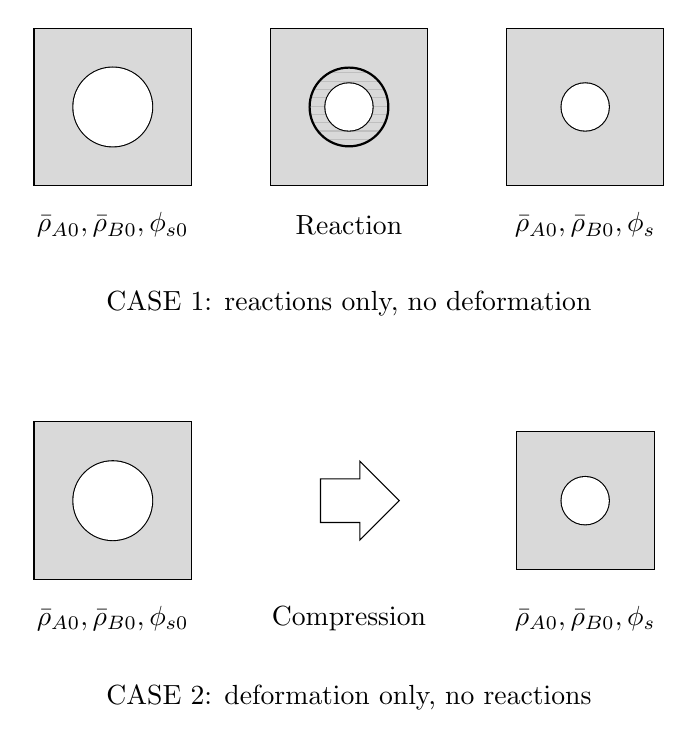
\begin{tikzpicture}[scale=1.0]
% Top row
% First square: with central hole
\node[draw, rectangle, minimum width=2cm, minimum height=2cm, fill=gray!30] (sq1) at (0,0) {};
\draw[thick, black] (0,0) circle (0.5cm); % Inner black line
\fill[white] (0,0) circle (0.5cm); % Hole
\node at (0,-1.5) {$\bar\rho_{A0}, \bar\rho_{B0}, \phi_{s0}$};
%
% Second square: with same hole but partial ring fill with black lines
\node[draw, rectangle, minimum width=2cm, minimum height=2cm, fill=gray!30] (sq2) at (3,0) {};
\fill[pattern=horizontal lines, pattern color=gray!50] (3,0) circle (0.5cm); % Hashed inner ring
%\fill[white] (3,0) circle (0.5cm); % Original hole
\draw[thick, black] (3,0) circle (0.5cm); % Outer black line
%\fill[gray!50] (3,0) circle (0.5cm); % Fill ring
\draw[thick, black] (3,0) circle (0.3cm); % Inner black line
\fill[white] (3,0) circle (0.3cm); % Smaller inner hole
\node at (3,-1.5) {Reaction};
\node at (3,-2.5) {CASE 1: reactions only, no deformation};
%
% Third square: with smaller hole
\node[draw, rectangle, minimum width=2cm, minimum height=2cm, fill=gray!30] (sq3) at (6,0) {};
\draw[thick, black] (6,0) circle (0.3cm); % Inner black line
\fill[white] (6,0) circle (0.3cm); % Smaller hole matching inner
\node at (6,-1.5) {$\bar\rho_{A0}, \bar{\rho}_{B0}, \phi_s$};
%
% Bottom row
% First square: with central hole
\node[draw, rectangle, minimum width=2cm, minimum height=2cm, fill=gray!30] (sq1) at (0,-5) {};
\draw[thick, black] (0,-5) circle (0.5cm); % Inner black line
\fill[white] (0,-5) circle (0.5cm); % Hole
\node at (0,-6.5) {$\bar\rho_{A0}, \bar\rho_{B0}, \phi_{s0}$};
%
% Arrow
\node[single arrow, draw, minimum width=1cm, minimum height=1cm, single arrow head extend=0.1cm, shape border rotate=0, anchor=center] (arrow2) at (3,-5) {};
\node at (3,-6.5) {Compression};
\node at (3,-7.5) {CASE 2: deformation only, no reactions};
%
% Third square: with smaller hole
\node[draw, rectangle, minimum width=1.75cm, minimum height=1.75cm, fill=gray!30] (sq3) at (6,-5) {};
\draw[thick, black] (6,-5) circle (0.3cm); % Inner black line
\fill[white] (6,-5) circle (0.3cm); % Smaller hole matching inner
\node at (6,-6.5) {$\bar\rho_{A0}, \bar{\rho}_{B0}, \phi_s$};
%
\end{tikzpicture}
\end{center}
\caption{The effect of porosity-filling reactions on solid volume fraction.  Gray denotes the load-bearing solid skeleton, white denotes pore fluid, and the hatched annulus denotes product solid that has precipitated into pore volume. CASE 1 changes the solid volume fraction by reaction at fixed skeleton deformation, while CASE 2 changes the same volume fraction by mechanical compression.}\label{fig:porosity-filling}
\end{figure}
%

Additionally, the reactive-transport and poromechanical models discussed above do not account for momentum production arising from reactions. In mixture theory this term is not an empirical body force: momentum is mass times velocity, so mass transferred from one phase to another carries momentum into the receiving phase at the velocity of that phase. If the donor and recipient phases move at different velocities, the transferred mass changes phase momentum and the phase momentum balances must account for the corresponding production or destruction. These same models also employ a standard Darcy relative flux that does not consistently account for fluid loss to reaction, leading to inconsistencies in the mass and momentum balances during reactive processes. More broadly, the reactive transport theories for porous media that we have surveyed \cite{steefel2015rt} do not include the thermodynamic driving force that follows from the reaction mass constraint. In the present formulation, that force appears naturally through the \emph{exchange potential} $\tau$, whose gradient enters a generalized Darcy law together with the fluid-loss term. The underlying $\nabla_{\mbf{x}}\tau$ contribution is already present in the Bedford--Drumheller variational theory of reacting immiscible mixtures~\cite{drumheller1980thermomechanical,drumheller2000}; the extension here is to carry it through the fluid momentum balance, define a relative mass flux, and obtain the corresponding Darcy-type closure. Direct experimental isolation of this term would require resolving flow and momentum exchange within active reaction fronts, where pressure gradients, permeability evolution, pore geometry, and reaction kinetics are strongly coupled. The theoretical requirement is nevertheless clear: the relative flux is not merely a standard Darcy law with a source term appended to the mass balance, but a constitutively modified flux that handles fluid consumption and thermodynamic driving forces in a consistent manner. Together, these shortcomings can lead to inaccurate predictions of fracture initiation, because the models do not distinguish between porosity-filling and stress-generating volume changes and do not properly capture reaction-induced momentum transfer or chemically driven fluid transport.

The special nature of hydration reactions during retrograde metamorphism has long been recognized and is exemplified by the serpentinization of ultramafic rocks \cite{macdonald1985}. Hydration reactions are characterized by a significant increase in solid volume and a protolith that has no detectable porosity. Jamtveit et al.\ \cite{jamtveit2000} recognized the importance of stress heterogeneities due to local volume increases that fracture the rock and allow fluid access. This process is generally referred to as reaction-driven cracking, and the broader geophysics literature on this process is now substantial. Kelemen and Hirth~\cite{kelemen2011reaction} showed that the volume change due to reaction can generate stresses sufficient to fracture rock during retrograde metamorphism, and Rudge et al.~\cite{rudge2010simple} demonstrated with a simplified model that cracking is required to explain observed serpentinization rates. Pl\"umper et al.~\cite{plumper2012serpentine} observed the fracturing mechanism directly at the nanoscale, and Malvoisin et al.~\cite{malvoisin2017serpentinization} quantified experimentally the feedback between reaction rate and fracture generation. Evans et al.~\cite{evans2020phasefield} further showed, using a phase-field fracture framework, how background stress, fluid pressure gradients, and chemical driving force can interact to control the extent of serpentinization. Taken together, these studies motivate a continuum theory that captures the full coupling among finite-strain mechanics, porosity evolution, reaction kinetics, and fluid transport.

Several theoretical frameworks for multiphase porous media at finite strains already exist. The Theory of Porous Media (TPM), developed by de~Boer~\cite{deboer2000theory} and Ehlers~\cite{ehlers2002foundations,ehlers2017challenges}, treats the porous medium as a superimposed continuum of immiscible phases with balance equations and thermodynamic restrictions in a finite-deformation setting. Coussy's poromechanical framework~\cite{coussy2004poromechanics,coussy2006deformation} provides a complementary energy-based approach applied to crystallization pressure and chemo-mechanical coupling. Borja and Alarc\'on~\cite{borja1995mathematical} and Borja~\cite{borja2006mechanical} developed variational and finite-strain formulations for elastoplastic consolidation within the Biot framework. The present work builds instead on the Bedford--Drumheller mixture theory~\cite{drumheller1980thermomechanical}, specifically Drumheller~\cite{drumheller2000}, who introduced the distention gradient as a kinematic variable that separates porosity-filling and microstructural reorienting volume changes from stress-generating ones. Unlike Coussy's framework, we work directly with phase-level free energies for elasticity and introduce a skeleton-level potential we call the \emph{distention energy} to account for grain reorientation and porosity changes. This is advantageous when the reaction products have elastic properties different from those of the reactants, because the effective mechanical properties of the skeleton update automatically via mixture rules as the reaction progresses---a feature absent from both the eigenstrain models of Evans et al.~\cite{evans2018}, Evans et al.~\cite{evans2020phasefield}, and Zhang et al.~\cite{zhang2025}, and from the standard reactive transport codes reviewed by Steefel et al.~\cite{steefel2015rt}, including TOUGHREACT~\cite{xu2011toughreact} and CrunchFlow~\cite{steefel1994crunch}. Those codes are powerful for chemistry and transport, but they do not provide the phase-level finite-strain mechanical framework required here.

This work presents a finite-deformation formulation for a reacting three-phase mixture comprising a fluid and two solid phases (reactant and product). Building on mixture theory~\cite{drumheller2000} and extending Biot poromechanics to finite strains~\cite{foster2025}, our model introduces a multiplicative decomposition of the deformation gradient into distention and true deformation phases. The distention gradient explicitly separates reaction-induced volume changes that consume porosity and reorient the microstructure from those that strain the mineral solids and potentially lead to failure, thereby correcting the assumption in prior models that all volume expansion generates stress. We also derive momentum production terms due to reactions and a generalized Darcy-like relative flux in which both fluid loss to reaction and the thermodynamic driving force associated with the exchange potential $\tau$ are handled consistently. The key contributions are:
\begin{itemize}
    \item Explicit coupling of reaction kinetics with finite-strain kinematics via the distention framework, ensuring that the conservation laws are satisfied in the reference configuration while allowing reactions to fill pores without necessarily generating stress.
    \item A generalized Darcy law for the relative fluid flux that consistently incorporates fluid consumption by reaction and the gradient of the exchange potential $\tau$, enabling chemically driven fluid transport in addition to pressure-driven flow.
    \item Weak forms suitable for numerical implementation, facilitating predictions of reaction-induced fracturing when coupled with fracture-initiation and propagation models, e.g.\ peridynamics \cite{agrawal2020coupling}, GFEM \cite{duarte2008analysis}, or phase-field methods \cite{wilson2016phase}.
\end{itemize}

This framework applies to reactions beyond serpentinization. For example, the hydration of anhydrite to gypsum involves a substantial volume increase of approximately 61\%~\cite{butscher2011}. Such swelling can cause fracturing in rock formations and even damage surface structures \cite{Sass_2010}, making it an ideal case for the model to predict stress evolution and failure in sulfate-rich environments, where the distention approach can distinguish porosity consumption from skeleton straining.

By addressing finite-deformation kinematics, the nuanced role of volume expansion in stress generation, and the effects of reaction on momentum and relative flux, this model provides a more rigorous tool for simulating mineral alteration and related geomechanical processes.


\section{Momentum balance}

The governing equations are obtained from Hamilton's extended principle for reacting immiscible mixtures; the full derivation is given in Appendix~\ref{sec:variational}.  In the present section we collect only the balance laws and constitutive relations needed in the main development.

The variational principle is
\[
  \int_{t_1}^{t_2}\left[\delta(T-U)+\delta W+\sum_k \delta C_k\right]dt = 0,
\]
where $T$ is the kinetic energy, $U$ is the internal energy, $\delta W$ is the virtual work of body and interaction forces, and $\delta C_k$ is the variation of $k$ constraint equations enforced by Lagrange multipliers.  The principal constraints introduced are
\begin{subequations}
\begin{align}
  \sum_\xi \phi_\xi &=1, \label{eq:sum_phi}\\
  \sum_\xi c^{+}_\xi &= 0, \label{eq:sum_cplus}\\
  J_\xi - \frac{\phi_{\xi 0}\bar\rho_{\xi 0}+c_\xi}{\phi_\xi\bar\rho_\xi} &= 0. \label{eq:phase_mass_constraint}
\end{align}
\end{subequations}
Equation~\eqref{eq:sum_phi} is the volume fraction constraint, where $\phi_\xi$ is the volume fraction of phase $\xi$.  Equation~\eqref{eq:sum_cplus} is the overall mixture mass balance, where $c_\xi^+=\dot c_\xi/J_\xi$ is the mass production rate per unit current mixture volume, $c_\xi$ is the mass added per unit reference volume by reaction, and $J_\xi$ is the Jacobian of the motion of phase $\xi$ defined below.  Equation~\eqref{eq:phase_mass_constraint} is the material mass balance for each phase including mass transfer, with $\bar\rho_\xi$ and $\bar\rho_{\xi 0}$ denoting the current and reference intrinsic densities and $\phi_{\xi 0}$ the reference volume fraction.  In addition, the interaction forces satisfy the standard mixture-theory identity
\begin{equation}
  \sum_\xi \mbf{b}_\xi = 0,
  \label{eq:sum_b}
\end{equation}

where $\mbf{b}_\xi$ is the interaction force exerted on phase $\xi$ by the others.  The partial density is $\rho_\xi = \phi_\xi\bar\rho_\xi$.  

We assume a continuously differentiable, one-to-one map between position vectors in the reference configuration $\mbf{X}_\xi$ and current configurations $\mbf{x}$ called the \emph{motion} $\bs{\chi}_\xi$
%
\[
  \mbf{x} = \bs{\chi}_\xi(\mbf{X}_\xi, t)
\]
%
The \emph{deformation gradient} of phase $\xi$ is
%
\[
  \mbf{F}_\xi = \frac{\partial \chi_\xi(\mbf{X}_\xi,t)}{\partial \mbf{X}_\xi}=\nabla_{\mbf{X}_\xi}\mbf{u}_\xi+\mbf{I},
\]
%
with Jacobian $J_\xi = \det(\mbf{F}_\xi)$.


We assume the solid phases share a common trajectory,
\[
  \bs{\chi}_A(\mbf{X}_A,t)=\bs{\chi}_B(\mbf{X}_B,t)=\bs{\chi}_s(\mbf{X}_s,t),
\]
while the fluid follows its own unique motion $\bs{\chi}_f$; see Fig.~\ref{fig:kinematics}.  


We use the spatial description of the material time derivative of a quantity $\square_\xi$ following the velocity of phase $\zeta$,
\[
  \frac{D_\zeta \square_\xi}{Dt} = \frac{\partial \square_\xi}{\partial t}+\mbf{v}_\zeta\cdot\nabla_{\mbf{x}}\square_\xi,
\]
and use the shorthand notation $\dot\square_\xi = D_\xi \square_\xi/Dt$ for the derivative following phase $\xi$.
%
\begin{figure}
\centering
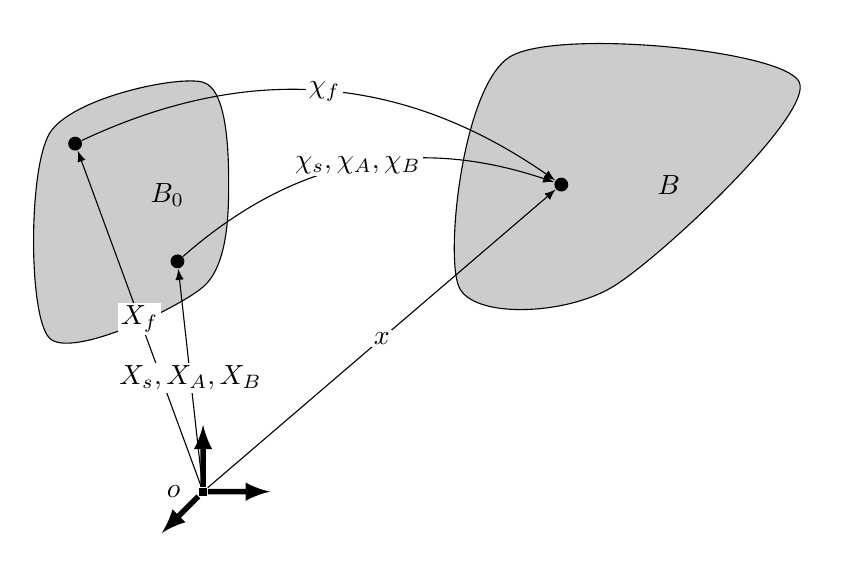
\begin{tikzpicture}[scale=0.65]
    \tikzstyle{pt}=[circle, fill=black, inner sep=0pt, minimum size=5pt]
    \draw [black, fill=black!20] plot [smooth cycle] coordinates {(-1.0,-1.0) (2,0) (2.5,2) (2,4) (-1,3)};
    \draw [black, fill=black!20] plot [smooth cycle] coordinates {(7, 0) (10,0) (13.65, 4) (8,4.5)};
    \draw (2,-4) node[fill=black, minimum size=3pt, inner sep=0pt, label={[label distance=3pt]180:$o$}] (O) {} ;
    \draw (-0.5,2.8) node[pt] (Xf) {} ;
    \draw (1.5,0.5) node[pt] (Xs) {} ;
    \draw (9.0,2) node[pt] (x) {} ;
    \draw[-latex] (O) -- (Xf) node[midway, fill=white, inner sep=1pt] {$\mbf{X}_f$} ;
    \draw[-latex] (O) -- (Xs) node[midway, fill=white, inner sep=1pt] {$\mbf{X}_s, \mbf{X}_A, \mbf{X}_B$} ;
    \draw[-latex] (O) -- (x) node[midway, fill=white, inner sep=1pt] {$\mbf{x}$} ;
    \draw[bend left, -latex] (Xs) to node[midway, fill=white, inner sep=1pt] {$\bs{\chi}_s,\bs{\chi}_A, \bs{\chi}_B$} (x);
    \draw[bend left, -latex] (Xf) to node[midway, fill=white, inner sep=1pt] {$\bs{\chi}_f$} (x);
    \draw (1.3,1.8) node () {${\mc{B}_0}$} ;
    \draw (11.1,2) node () {${\mc{B}}$} ;
    \draw (3.5,-4) node (xaxis) {} ;
    \draw (2,-2.5) node (yaxis) {} ;
    \draw (1.0,-5.0) node (zaxis) {} ;
    \draw[-latex, line width=2pt] (O) -- (xaxis)  {} ;
    \draw[-latex, line width=2pt] (O) -- (yaxis)  {} ;
    \draw[-latex, line width=2pt] (O) -- (zaxis)  {} ;
\end{tikzpicture}
\caption{Schematic description of kinematics showing the deformation maps, $\chi_\xi$, linking the reference configurations, $\mbf{X}_\xi$, to the current configurations, $\mbf{x}$. Note that we assume that the two phases of the solid mixture have the same deformation, $\chi_s$, and hence the same material configuration, $\mbf{X}_s$.}
\label{fig:kinematics}
\end{figure}
%

For the fully saturated three-phase system considered here, the porosity is the fluid volume fraction, i.e.\ $\phi = \phi_f$.  

The fluid momentum balance obtained from the Euler--Lagrange equations associated with the complete variational principle derived in Appendix~\ref{sec:variational} is
\begin{equation}
  \rho_f\mbf{a}_f = \rho_f\mbf{g} + \mbf{b}_f - \phi\nabla_{\mbf{x}}\bar p_f + c_f^+\left(\nabla_{\mbf{x}}\tau-\mbf{v}_f\right),
  \label{eq:fluid_momentum}
\end{equation}
where $\mbf{a}_f$ is the fluid acceleration, $\mbf{g}$ is gravity, $\mbf{b}_f$ is the interaction force on the fluid, and $\tau$ is the Lagrange multiplier associated with the mixture mass balance~\eqref{eq:sum_cplus} which we call the \emph{exchange potential}.  The fluid carries no deviatoric effective stress so its mechanical contribution enters through pressure and density changes only.

The last term in~\eqref{eq:fluid_momentum} is the reaction momentum-production term.  It appears because mass transferred into or out of the fluid phase carries momentum and must enter the phase momentum balance at the velocity of the phase into which the mass is assigned.  If mass leaves one phase moving with velocity $\mbf{v}_\xi$ and enters another moving with a different velocity, the phase momenta change even when the total mass transfer satisfies~\eqref{eq:sum_cplus}.  The contribution $c_f^+\nabla_{\mbf{x}}\tau$ is the force associated with the reaction mass constraint, while $-c_f^+\mbf{v}_f$ is the corresponding convective momentum carried by produced or consumed fluid mass.  This term has the same variational origin as the $\tau$ contribution in Bedford and Drumheller~\cite{drumheller1980thermomechanical}; here it is retained explicitly so that it can be propagated into the relative-flux closure.  Thus, when no reaction occurs ($c_f^+=0$), the term vanishes; when reaction consumes or produces fluid, the term is required for consistency between phase mass balance, phase momentum balance, and total mixture momentum.

Adding the solid and fluid balances gives the overall momentum balance
%
\begin{equation}
  \rho\mbf{a} = \nabla_{\mbf{x}}\cdot\left(\bs\sigma_s' - \bar p_f \mbf{I}\right) - \nabla_{\mbf{x}}\left[(1-\phi)p^\star_\phi\right] + \rho\mbf{g} - c_f^+\left(\mbf{v}_f-\mbf{v}_s\right),
  \label{eq:overall_mom}
\end{equation}
%
where $\rho_s = \rho_A+\rho_B$, $\rho = \rho_s+\rho_f$, $\bs\sigma_s' = \bs\sigma_A'+\bs\sigma_B'$ is the total solid effective Cauchy stress, and $\rho\mbf{a}=\rho_s\mbf{a}_s+\rho_f\mbf{a}_f$ is the mixture acceleration.  The additional term $\nabla_{\mbf{x}}[(1-\phi)p^\star_\phi]$ is the macroscopic consequence of the porosity-dependent solid free energy. $p^\star_\phi$ is the \emph{porosity-conjugate pressure} and will be discussed in more detail in section \S~\ref{sec:constitutive}. 

\subsection{Relative flux vector}
The relative mass flux of the fluid with respect to the solid is defined by
\[
  \mbf{w} = \phi\bar\rho_f(\mbf{v}_f-\mbf{v}_s),
\]
which is the fluid mass flow rate per unit current area measured in the solid frame.  Solving for the fluid velocity gives
\begin{equation}
  \mbf{v}_f = \mbf{v}_s + \frac{\mbf{w}}{\phi\bar\rho_f}.
  \label{eqn:rel_flux}
\end{equation}
Here $\mbf{v}_s$ is the material velocity of the load-bearing solid skeleton and $\mbf{v}_f$ is the pore-fluid velocity.
To close the fluid momentum balance, we adopt the standard linear drag form for the interaction force,
\[
  \mbf{b}_f = -\frac{\mu_f\phi}{\bar\rho_f}\mbf{k}^{-1}\mbf{w},
\]
where $\mbf{k}$ is the permeability tensor and $\mu_f$ is the fluid viscosity.  Substituting this relation and~\eqref{eqn:rel_flux} into~\eqref{eq:fluid_momentum} yields
\begin{align}
  \frac{\mu_f\phi}{\bar\rho_f}\mbf{k}^{-1}\mbf{w}
    &= \rho_f(\mbf{g}-\mbf{a}_f) - \phi\nabla_{\mbf{x}}\bar p_f + c_f^+\left(\nabla_{\mbf{x}}\tau-\mbf{v}_s-\frac{\mbf{w}}{\phi\bar\rho_f}\right), \notag\\
  \frac{1}{\rho_f}\left(\phi^2\mu_f\mbf{k}^{-1}+c_f^+\mbf{I}\right)\mbf{w}
    &= \rho_f(\mbf{g}-\mbf{a}_f) - \phi\nabla_{\mbf{x}}\bar p_f + c_f^+\left(\nabla_{\mbf{x}}\tau-\mbf{v}_s\right). \notag
\end{align}
Defining
\[
  \tilde{\mbf{k}} = \left(\phi^2\mu_f\mbf{k}^{-1}+c_f^+\mbf{I}\right)^{-1},
\]
we obtain the resulting generalized Darcy's law,
%
\begin{empheq}[box=\fbox]{equation}
  \mbf{w} = \rho_f\tilde{\mbf{k}}\left(\rho_f(\mbf{g}-\mbf{a}_f) - \phi\nabla_{\mbf{x}}\bar p_f + c_f^+\left(\nabla_{\mbf{x}}\tau-\mbf{v}_s\right)\right).
  \label{eq:reacting_flux}
\end{empheq}
%
The first two terms in~\eqref{eq:reacting_flux} are the usual body-force and pressure-gradient contributions, while the modified mobility tensor $\tilde{\mbf k}$ and the last term together constitute the reaction-induced correction: it accounts simultaneously for fluid loss to reaction through $c_f^+$ and for the exchange-potential driving force through $\nabla_{\mbf{x}}\tau$.  The correction is expected to matter most where reactions are spatially localized, because steep reaction fronts produce large gradients in the thermodynamic fields entering $\tau$ and concentrate interphase mass transfer over a small region.  Direct experimental isolation of this contribution is difficult for the same reason: it requires resolving fluid motion, reaction rate, pressure, and evolving pore geometry within the active front. 

In the absence of reactions ($c_f^+=0$) and under creeping-flow conditions ($\mbf{a}_f=\mbf{0}$), \eqref{eq:reacting_flux} reduces to the standard Darcy law,
\[
  \phi(\mbf{v}_f-\mbf{v}_s) = \frac{\mbf{k}}{\mu_f}\left(\bar\rho_f\mbf{g}-\nabla_{\mbf{x}}\bar p_f\right).
\]
The modified mobility $\tilde{\mbf{k}}$ remains positive-definite provided every eigenvalue of $\phi^2\mu_f\mbf{k}^{-1}+c_f^+\mbf{I}$ is positive.  If $c_f^+>0$ this condition is automatically strengthened relative to standard Darcy flow; if the reaction consumes fluid ($c_f^+<0$), it requires $|c_f^+|<\phi^2\mu_f/k_{\max}$, where $k_{\max}$ is the largest eigenvalue of $\mbf{k}$.  For geologically relevant parameters ($k\sim10^{-18}$--$10^{-15}$~m$^2$, $\phi\sim0.1$, $\mu_f\sim10^{-3}$~Pa$\cdot$s), this threshold is many orders of magnitude larger than typical reaction rates \cite{huang2019,cotellucci2024}, so the correction is well-conditioned in practice.  If this condition were violated, the linear drag closure would predict a negative mobility and the model should be interpreted as outside the range of validity of the assumed Darcy-scale closure rather than as a physically admissible material response.  Mathematically, one would then need a different dissipative closure or a regularized nonequilibrium reaction--transport model.

For the weak forms developed later it is convenient to pull the flux back to the solid reference configuration.  Neglecting fluid inertia in the flux law ($\mbf{a}_f=\mbf{0}$), we define the reference configuration relative flux and permeability by
\begin{equation}
  \mbf{W} = J_s\mbf{F}_s^{-1}\mbf{w},
  \qquad
  \tilde{\mbf{K}} = J_s\mbf{F}_s^{-1}\tilde{\mbf{k}}\mbf{F}_s^{-T},
 \label{eq:W material}
\end{equation}
and obtain
\begin{equation}
  \mbf{W} = \rho_f\tilde{\mbf{K}}\left(\rho_f\mbf{F}_s^T\mbf{g} - \phi\nabla_{\mbf{X}_s}\bar p_f + c_f^+\left(\nabla_{\mbf{X}_s}\tau-\mbf{F}_s^T\mbf{v}_s\right)\right).
  \label{eq:reacting_flux_ref}
\end{equation}

\subsection{Momentum balance in the reference configuration}
Finally, under quasi-static conditions ($\mbf{a}=\mbf{0}$), we pull back the overall momentum balance~\eqref{eq:overall_mom} to the reference configuration of the solid.  Writing the solid effective stress in terms of the first Piola--Kirchhoff stress $\mbf{P}_s'$ gives
%
\begin{equation}
  \mbf{0} = \nabla_{\mbf{X}_s}\cdot\left(\mbf{P}_s' - \bar p_f J_s\mbf{F}_s^{-T} - (1-\phi)p_\phi^\star J_s\mbf{F}_s^{-T}\right) + J_s\rho\mbf{g} - \frac{c_f^+}{\phi\bar\rho_f}\mbf{F}_s\mbf{W}.
  \label{eqn:final_momentum}
\end{equation}
%
where
%
\begin{equation*}
  \mbf{P}^\prime_s = J_s \bs{\sigma}^\prime_s \mbf{F}_s^{T}.
\end{equation*}
%

When $p_\phi^\star=0$ and in the absence of reactions $c^{+}_f =0$, this reduces to the standard pressure-coupled Terzaghi momentum balance \cite{sun2013stabilized} with incompressible mineral grains.

\section{Constitutive modeling}
\label{sec:constitutive}

We follow the kinematic framework of Drumheller \cite{drumheller2000} and adopt a multiplicative decomposition of the deformation gradient, i.e.\
%
\begin{equation}
  \mathbf{F}_\xi = \mathbf{A}_\xi \mathbf{\bar{F}}_\xi,
  \label{eq:mult_decomp_F}
\end{equation}
%
where $\mbf{A}_\xi$ is called the \emph{distention gradient} and $\mbf{\bar{F}}_\xi$ is the \emph{true deformation gradient}.  Computing the determinant of both sides of \eqref{eq:mult_decomp_F}
%
\begin{align}
  \det(\mathbf{F}_\xi) &= \det(\mathbf{A}_\xi) \det(\mathbf{\bar{F}}_\xi) \notag \\
  J_\xi &= \alpha_\xi \bar{J}_\xi,
  \label{eq:distention}
\end{align}
%
where $\alpha_\xi = \det(\mathbf{A}_\xi)$ is called the \emph{distention}.  In order to determine $\bar{J}_\xi$ we need to determine $\alpha_\xi$ which will require an additional evolution equation. Consider the material form of conservation of mass for phase $\xi$
%
\begin{align}
  J_\xi \phi_{\xi} \bar\rho_{\xi} = \phi_{\xi 0} \bar\rho_{\xi 0} + c_\xi.
  \label{eq:material_mass}
\end{align}
%
Substitute \eqref{eq:distention} into \eqref{eq:material_mass} and require $\bar{J}_\xi = {\bar{\rho}_{\xi 0}} / {\bar\rho_\xi}$ which is the \emph{true (local) conservation of mass}, this gives
%
\begin{align}
  \alpha_\xi \phi_{\xi}\bar\rho_{\xi 0}  - \phi_{\xi 0}\bar\rho_{\xi 0} =    c_\xi. \label{eq:material_mass_distention}
\end{align}
%
Equation~\eqref{eq:material_mass_distention} demonstrates that the volume fraction is only uniquely related to the motion in the absence of mass exchange.  The adjective ``true'' is used here in Drumheller's sense: $\bar{J}_\xi$ measures the volume change of the phase material itself, not the volume change of the mixture volume occupied by that phase.  Thus $\bar{J}_\xi=\bar\rho_{\xi0}/\bar\rho_\xi$ follows from local conservation of mass for the intrinsic phase material, whereas the product $\alpha_\xi\phi_\xi$ accounts for pore filling, grain rearrangement, and mass exchange with the other phases. Taking the natural log of both sides of \eqref{eq:distention} and then the material time derivative provides an evolution law for the distention.
%
\begin{align}
  \frac{\dot{\alpha}_\xi}{\alpha_\xi}  &= \frac{\dot{\bar\rho}_\xi}{\bar\rho_\xi} + \nabla_{\mathbf{x}} \cdot \mbf{v}_\xi \label{eq:dist_evo}
\end{align}
%
For the incompressible reactant and product $\dot{\bar\rho}_A = \dot{\bar\rho}_B = 0$ and both follow the trajectory of the solid, therefore evaluating \eqref{eq:dist_evo} for $\xi = s$ gives
%
\begin{align}
  \dot{\alpha}_s &= {\alpha_s} \nabla_{\mathbf{x}} \cdot \mbf{v}_s \notag
\end{align}
%
Substituting the well-known identity $\dot{J}_s = J_s \nabla_{\mbf x} \cdot \mbf{v}_s$ and rearranging gives
%
\begin{align}
  \frac{\dot{\alpha}_s}{\alpha_s} &=  \frac{\dot{J}_s}{J_s}.  \label{eq:dist_evo2}
\end{align}
%
Inspecting \eqref{eq:dist_evo2} it's evident that for incompressible solid phases
%
\begin{align}
  \alpha_s &=  J_s,  \label{eq:dist_evo3}
\end{align}
%
and therefore we can eliminate the need to solve for $\alpha_s$ by explicitly using $J_s$ in its place for the incompressible-solid simulations in this paper.  In that setting the distention is not an additional primary unknown in the finite element implementation.  The novelty is the way the distention framework identifies the part of the free energy associated with true shape change, $\mbf{\bar F}_s$, separately from the skeleton volumetric response, so that porosity changes at fixed $J_s$ do not generate hydrostatic stress.  If compressible grains are allowed, then $\dot{\bar\rho}_s/\bar\rho_s$ in~\eqref{eq:dist_evo} need not vanish, $\alpha_s\neq J_s$, and an independent constitutive law or evolution equation for intrinsic density or distention would be required.

Drumheller \cite{drumheller2000} demonstrates that at most the distention gradient can change the distention $\alpha_\xi$ and cause a simple rotation of the material.  From the tensor polar decomposition we have
%
\begin{align}
  \mbf{A}_\xi = \alpha_\xi^{\nicefrac{1}{3}} \mathbf{R}_\xi, \notag
\end{align}
%
where $\mathbf{R}_\xi$ is an orthonormal rotation tensor; however, in heterogeneous materials\footnote{i.e.\ those with disordered microstructure such that structured grain reorientation during reactions is not expected} it's reasonable to assume $\mathbf{R}_\xi = \mbf{I}$, thus
%
\begin{align}
  \mbf{A}_\xi = \alpha_\xi^{\nicefrac{1}{3}} \mathbf{I}, \notag
\end{align}
%
and
%
\begin{align}
  \mbf{\bar F}_\xi = \alpha_\xi^{-\nicefrac{1}{3}} \mathbf{F}_\xi. \notag
\end{align}
%
Importantly, given the equivalence of $\alpha_s$ and $J_s$, we have
%
\begin{align}
  \mbf{\bar F}_s = J_s^{-\nicefrac{1}{3}} \mathbf{F}_s.
  \label{eq:Fbar}
\end{align}
%
An important consequence of~\eqref{eq:Fbar} is that the true Jacobian satisfies
%
\begin{align*}
  \bar{J}_s = \det\left(\mbf{\bar F}_s\right) = J_s^{-1} J_s = 1 \quad \text{(identically)}.
\end{align*}
%
The incompressibility of the individual solid mineral phases in the distention formulation is therefore a kinematic identity---no separate constraint equation, penalty, or Lagrange multiplier is required.

\paragraph{Remark.}  For incompressible solid phases the decomposition~\eqref{eq:mult_decomp_F} combined with the assumption $\mbf{R} = \mbf{I}$ reduces kinematically to the classical volumetric--isochoric multiplicative split~\eqref{eq:Fbar} (cf.\ \cite{flory1961}), with $\mbf{A}_s = J_s^{\nicefrac{1}{3}}\mbf{I}$ playing the role of the volumetric part.  The kinematics are therefore equivalent to the standard decomposition when $\alpha_s = J_s$; however, we retain the full distention framework of Drumheller~\cite{drumheller2000} for two reasons.  First, it motivates the decomposition of the free energies into an isochoric part and a distention part, allowing the strain energy to depend on $J_s$ and $\phi$ through \emph{independent} paths and thereby distinguish porosity-filling volume changes from stress-generating ones (cf.\ Fig.~\ref{fig:porosity-filling}).  Second, it extends naturally to compressible solid phases, for which $\alpha_s \neq J_s$ and the distention evolves independently of the deformation, or to cases of structured grain reorientation during reactions for which $\mbf{R} \ne \mbf{I}$.

We write the strain energy density as
%
\begin{equation}
  W_\xi(\mbf{F}_s, \phi) = W^{\text{iso}}_\xi(\mbf{\bar F}_s) + W^{\text{dis}}_\xi(J_s, \phi),
  \label{eq:W_decomp}
\end{equation}
%
with $W_\xi = \rho_{\xi 0} \psi_\xi $, where $W^{\text{iso}}_\xi(\mbf{\bar F}_s)$ is the isochoric elastic strain energy representing the shape-change response of individual mineral grains and $W^{\text{dis}}_\xi(J_s, \phi)$ is the \emph{distention energy} representing the volumetric response of the porous microstructure.  $\psi_\xi$ is the Helmholtz free energy of phase $\xi$. The distention energy captures the energetic cost of rearranging incompressible mineral grains within the skeleton and provides the macroscopic bulk modulus; it is distinct from the (vanishing) mineral compressibility energy.  The explicit $\phi$-dependence introduces inter-phase body forces in the variational principle (Appendix~\ref{sec:variational}) and a correction to the distention stress in the Coleman--Noll procedure (Appendix~\ref{sec:coleman}).

Computing $\dot\psi_\xi$ in the entropy inequality requires the chain rule through all three paths ($\mbf{\bar F}_s$, $J_s$, and $\phi$)
%
\begin{equation}
  \left.\p{W_\xi}{F_{kl}}\right\vert_\phi = \p{W^{\text{iso}}_\xi}{\bar{F}_{mn}} \frac{\partial \bar{F}_{mn}}{\partial F_{kl}} + \left.\frac{\partial W_\xi^{\text{dis}}}{\partial J_s}\right\vert_\phi\, J_s\, F^{-T}_{kl},
  \label{eq:chain_rule_both}
\end{equation}
%
where the fourth-order tensor
%
\begin{align}
  \frac{\partial \bar{F}_{ij}}{\partial F_{kl}} = J_s^{-\nicefrac{1}{3}}\left(\delta_{ik}\delta_{jl} - \frac{1}{3} F_{ij} F^{-T}_{kl}\right)
  \label{eq:chain_rule_Fbar}
\end{align}
%
carries a deviatoric projection: the subtracted term $-\frac{1}{3}F_{ij}F^{-T}_{kl}$ arises from differentiating the $J_s^{-\nicefrac{1}{3}}$ prefactor and ensures that the isochoric contribution to the stress has zero hydrostatic content.  The second term in~\eqref{eq:chain_rule_both} uses $\partial J_s / \partial F_{kl} = J_s F^{-T}_{kl}$.  As shown in Appendix~\ref{sec:coleman}, requiring the entropy inequality to hold for arbitrary $\dot{\mbf{F}}_s$ yields the effective first Piola--Kirchhoff stress of the solid mixture
%
\begin{align}
  \mbf{P}'_s = \sum_{\xi=A,B}\left[{J_s^{\nicefrac{2}{3}}  \phi_\xi \left(\mbf{\bar P}'_\xi - \frac{1}{3}\left(\mbf{\bar P}'_\xi : \mbf{F}_s\right) \mbf{F}_s^{-T}\right)} + \phi_\xi{\bar{p}_\xi^\star J_s\, \mbf{F}_s^{-T}}\right],
  \label{eq:P_projected}
\end{align}
%
where $\mbf{\bar p}'_\xi = \partial W^{\text{iso}}_\xi / \partial\mbf{\bar F}_s$ is the \emph{undistended intrinsic first Piola--Kirchhoff effective stress}, i.e.\ the stress that an isolated mineral grain with deformation $\mbf{\bar F}_s$ would experience, and
%
\begin{equation}
  \bar{p}^\star_\xi = \left.\frac{\partial W_\xi^{\text{dis}}}{\partial J_s}\right\vert_\phi + \frac{1-\phi}{J_s}\left.\frac{\partial W_\xi^{\text{dis}}}{\partial \phi}\right\vert_{J_s}
  \label{eq:Kstar_def}
\end{equation}
%
is the $\xi$-phase skeleton (mineral solid plus pore space) porosity-conjugate pressure.  The corresponding Cauchy effective stress is
%
\begin{align}
  \bs\sigma'_s = \frac{1}{J_s}\mbf{P}'_s \mbf{F}_s^T.
  \label{eq:cauchy_projected}
\end{align}
%
The deviatoric (isochoric) contribution to~\eqref{eq:cauchy_projected} is traceless by construction, while the distention energy provides the hydrostatic response of the skeleton.

\subsection{Specific form of constitutive model}
%
We now specialize the constitutive model by choosing explicit forms for the isochoric and distention parts of the free energy in~\eqref{eq:W_decomp}.  For the isochoric contribution we adopt a neo-Hookean model,
%
\begin{align}
  W^{\text{iso}}_\xi(\mbf{\bar F}_s) = \frac{G_\xi}{2}\left(\mbf{\bar F}_s : \mbf{\bar F}_s - 3\right) = \frac{G_\xi}{2}\left(J_s^{-\nicefrac{2}{3}} I_1 - 3\right),
\end{align}
%
where $I_1 = \mbf{F}_s : \mbf{F}_s$ and $G_\xi$ is the shear modulus of phase $\xi$. For the distention contribution we choose the logarithmic form
%
\begin{equation}
  W^{\text{dis}}_\xi(J_s,\phi) = \frac{K^\star_\xi}{2(1-\phi)}\left(\ln J_s\right)^2,
  \label{eq:U_distention}
\end{equation}
%
where $K^\star_\xi$ is the distention modulus associated with phase $\xi$.  This term represents the energetic cost of changing the volume of the porous skeleton by rearranging incompressible mineral grains and pore space; it is therefore a skeleton-level bulk response, not a mineral compressibility energy.  The explicit factor $(1-\phi)^{-1}$ reflects the dependence of that volumetric response on the current load-bearing solid fraction.

The explicit $\phi$-dependence in \eqref{eq:U_distention} does not imply that porosity changes alone generate stress: if $J_s=1$, then $\ln J_s = 0$ and the distention contribution vanishes even if $\phi$ evolves.  Rather, the role of $\phi$ is to let the volumetric constitutive response of the skeleton depend on the current pore geometry and to generate the porosity-conjugate term $p_\phi^\star$ in the momentum balance.

For the neo-Hookean choice above, the undistended intrinsic first Piola--Kirchhoff stress is
%
\[
  \mbf{\bar P}'_\xi = \frac{\partial W^{\text{iso}}_\xi}{\partial \mbf{\bar F}_s} = G_\xi \mbf{\bar F}_s = G_\xi J_s^{-\nicefrac{1}{3}}\mbf{F}_s.
\]
%
For the distention energy~\eqref{eq:U_distention}, the scalar porosity-conjugate pressure defined in~\eqref{eq:Kstar_def} becomes (see Appendix~\ref{sec:coleman}, Eq.~\eqref{eq:Pstar_explicit})
%
\begin{equation}
  \bar p^\star_\xi = \frac{K_\xi^\star}{(1-\phi)J_s}\ln J_s\left(1+\frac{1}{2}\ln J_s\right).
\end{equation}
%
Substituting these expressions into~\eqref{eq:P_projected} yields the effective first Piola--Kirchhoff stress of the solid mixture,
%
\begin{align*}
  \mbf{P}'_s = G_{\text{eff}} J_s^{\nicefrac{1}{3}}\left[\mbf{F}_s - \frac{1}{3}I_1\mbf{F}_s^{-T}\right] + K_{\text{eff}}^\star\ln J_s\left(1+\frac{1}{2}\ln J_s\right)\mbf{F}_s^{-T},
\end{align*}
%
where, as a result of the derivation, we have a simple linear volume-fraction weighting for the effective properties
\begin{equation}
  G_{\text{eff}} = \phi_A G_A + \phi_B G_B,
\end{equation}
%
and
\begin{equation}
  K^\star_{\text{eff}} = \frac{1}{1-\phi}\left(\phi_A K_A^\star + \phi_B K_B^\star\right).
  \label{eq:K_star_mixture}
\end{equation}
In the single-solid limit ($\phi_B = 0$), \eqref{eq:K_star_mixture} reduces to $K_{\text{eff}}^\star = K_A^\star$, independent of porosity.  This is consistent with interpreting $K_\xi^\star$ as a calibrated skeleton parameter associated with phase $\xi$, while the factor $(1-\phi)^{-1}$ converts the volume-fraction weighting into a weighting by load-bearing solid fraction.

The corresponding effective Cauchy stress is
%
\begin{align*}
  \bs\sigma'_s = G_{\text{eff}}J_s^{-\nicefrac{2}{3}}\mbox{dev}(\mbf{B}_s) + \frac{K_{\text{eff}}^\star\ln J_s}{J_s}\left(1+\frac{1}{2}\ln J_s\right)\mbf{I},
\end{align*}
%
where $\mbf{B}_s = \mbf{F}_s\mbf{F}_s^T$.  The first term is traceless by construction, while the second term provides the macroscopic hydrostatic response of the porous skeleton.  The factor $\left(1+\frac{1}{2}\ln J_s\right)$ changes sign only for $J_s < e^{-2} \approx 0.135$, corresponding to extreme compression well beyond the regime of interest for almost all materials.

\paragraph{Plane-strain specialization.}  For two-dimensional plane strain simulations presented in the following sections with $F_{33} = 1$, the three-dimensional first invariant is $I_1^{3\text{D}} = \mbf{F}_s:\mbf{F}_s\vert_{2\text{D}} + 1$ and $J_s = \det_{2\text{D}}(\mbf{F}_s)$.

\paragraph{Remark (deviatoric projection).}  The deviatoric projection in the first term of~\eqref{eq:P_projected}---arising naturally from the chain rule through $\mbf{\bar F}_s(\mbf{F}_s)$ in the Coleman--Noll procedure (Appendix~\ref{sec:coleman})---ensures that no isochoric deformation generates hydrostatic stress.  The skeleton's volumetric response enters entirely through the distention energy $W^{\text{dis}}_\xi(J_s, \phi)$, which provides a finite bulk modulus $K^\star_{\text{eff}}$ that is typically much smaller than the mineral bulk modulus $K_s \to \infty$.  In Appendix~\ref{sec:biot} we show that this formulation reduces to standard Biot poromechanics with Biot coefficient $B = 1$ and skeleton bulk modulus $K = K^\star_{\text{eff}}$ when reactions are absent.

\paragraph{Remark (crystallization pressure).} The distention energy $W^{\text{dis}}_\xi(J_s, \phi)$ provides a natural mechanism for \emph{crystallization pressure}---the stress that develops when minerals grow in a confined space~\cite{correns1949growth, scherer1999crystallization}.  Classical treatments derive the maximum crystallization pressure from thermodynamics: Correns~\cite{correns1949growth} showed that the stress a growing crystal can exert on a confining wall is bounded by $\sigma_c = (RT / V_m) \ln \Omega$, where $\Omega$ is the supersaturation ratio and $V_m$ is the molar volume of the crystal.  Subsequent work by Scherer~\cite{scherer1999crystallization} and Steiger~\cite{steiger2005crystal} refined these estimates to account for interfacial curvature and pore geometry.  These approaches give the \emph{thermodynamic driving force} for crystallization pressure but do not, by themselves, describe the macroscopic mechanical response of the porous skeleton.

Coussy~\cite{coussy2006deformation} addressed this gap by embedding crystallization within a poromechanical framework, introducing a crystal pore pressure $p_c$ alongside the fluid pressure $\bar{p}_f$.  His momentum balance takes the form
%
\[
  \nabla \cdot \bs\sigma'' - B\,\nabla \bar{p}_f - B_c \nabla p_c + \rho\,\mbf{g} = \mbf{0},
\]
%
where $B_c$ is a crystal Biot coefficient.  The porosity-conjugate pressure $p^\star_\phi$ in the present theory~\eqref{eq:overall_mom} plays a structurally analogous role to Coussy's $p_c = -\phi p^\star_{\phi}$ with $B = B_c = 1$.

A key distinction is in how the two frameworks separate chemistry from mechanics.  In Coussy's approach, $p_c$ is determined by the supersaturation of the pore solution and the crystal--liquid interfacial energy---it is a thermodynamic quantity that persists even at infinitesimal strains.  In the present theory, the thermodynamic driving force for the reaction (supersaturation, chemical affinity) enters through $\tau$ and the reaction kinetics, while the \emph{mechanical consequence} of crystal growth in confinement is handled entirely by the distention energy $W^{\text{dis}}_\xi(J_s, \phi)$ and the porosity-conjugate pressure $p^\star_\phi$.  This cleanly separates what drives the reaction (chemistry, encoded in $\tau$) from what stress results (mechanics, encoded in $W^{\text{dis}}$ and $p^\star_\phi$).  Note that $p^\star_\phi$ is $O(\varepsilon^2)$ in the small-strain limit (see Appendix~\ref{sec:biot}, Eq.~\eqref{eq:Pstar_phi_explicit}).  This is physically consistent: in a porous medium, crystallization pressure generates macroscopic skeleton stress only when the growing solid phase fills the available pore space and further growth requires displacing the pore walls, i.e.\ $J_s \neq 1$.  Until the volumetric changes become significant, the crystal simply fills void space without stressing the skeleton.  The Biot coupling with $\bar{p}_f$ then determines the partitioning between fluid pressure changes and skeleton stress, while the modified Darcy flux~\eqref{eq:reacting_flux} controls how rapidly fluid transport can adjust to the pressure changes.


\section{Mass balances}
For a $\xi$ phase in the mixture, the mass balance \eqref{eq:material_mass_distention} can be written in the current configuration as
% \[
%   \frac{\partial \rho_\xi}{\partial t} + \nabla_{\mathbf{x}} \cdot \left(\rho_\xi \mathbf{v}_\xi\right) = c^{+}_\xi.
% \]
%
% Substituting $\rho_\xi = \phi_\xi \bar{\rho}_\xi$ gives
\[
  \frac{\partial \left(\phi_\xi \bar\rho_\xi\right)}{\partial t} + \nabla_{\mathbf{x}} \cdot \left(\phi_\xi \bar\rho_\xi \mathbf{v}_\xi\right) = c^{+}_\xi,
\]
where $\rho_\xi = \phi_\xi \bar{\rho}_\xi$.
%
We assume $\phi_f = \phi$ (i.e.\ the porosity) and the reactant ($A$) and product ($B$) phases to be incompressible; this gives the following mass balance equations for each phase in the mixture
%
\begin{subequations}
\begin{align}
  \frac{\partial \left(\phi \bar\rho_f\right)}{\partial t} + \nabla_{\mathbf{x}} \cdot \left(\phi \bar\rho_f \mathbf{v}_f\right) &= c^{+}_f, \label{eq:mass_f} \\
  \frac{\partial \phi_A }{\partial t} + \nabla_{\mathbf{x}} \cdot \left(\phi_A  \mathbf{v}_s\right) &= \frac{c^{+}_A}{\bar\rho_A}, \label{eq:mass_A} \\
  \frac{\partial \phi_B }{\partial t} + \nabla_{\mathbf{x}} \cdot \left(\phi_B  \mathbf{v}_s\right) &= \frac{c^{+}_B}{\bar\rho_B}, \label{eq:mass_B}
\end{align}
  \label{eq:mass_all}
\end{subequations}
where $c_\xi^+=\dot c_\xi/J_s$ is the mass production rate per unit current mixture volume, and $\dot{c}_\xi$ is the mass production rate per unit solid reference volume.

\subsection{Fluid mass balance}
Substituting the relative mass flux of the fluid \eqref{eqn:rel_flux} into \eqref{eq:mass_f} we obtain the fluid mass balance equation in the current configuration
%
% \begin{equation*}
%   \frac{\partial (\phi_f \bar{\rho}_f)}{\partial t} + \nabla_{\mathbf{x}} \cdot \left( \phi_f \bar{\rho}_f \left( \mathbf{v}_s + \frac{\mathbf{w}}{\phi_f \bar{\rho}_f} \right) \right) = c^{+}_f.
% \end{equation*}
% %
% Distributing the terms inside the divergence
% and using the linearity of the divergence operator, we split it as
%
\begin{equation*}
\frac{\partial (\phi_f \bar{\rho}_f)}{\partial t} + \nabla_{\mathbf{x}} \cdot (\phi_f \bar{\rho}_f \mathbf{v}_s) + \nabla_{\mathbf{x}} \cdot \mathbf{w} = c^{+}_f.
\end{equation*}
%
Here we have separated the contributions of the solid motion and the relative fluid flux. This allows us to introduce the material derivative following the solid to write
%
\begin{equation}
  \frac{D_s}{Dt} (\phi_f \bar{\rho}_f) + \phi_f \bar{\rho}_f \nabla_{\mathbf{x}} \cdot \mathbf{v}_s + \nabla_{\mathbf{x}} \cdot \mathbf{w} = c^{+}_f \label{eqn:mass_temp}.
\end{equation}
%
The divergence of the solid velocity can be eliminated using the identity $\dot{J}_s = J_s \nabla_{\mathbf{x}} \cdot \mathbf{v}_s$. After dividing by $J_s$ we obtain the following form of the mass balance
% To introduce the constitutive equation for the fluid we observe the following
%
% \begin{align}
%   \frac{D_s}{Dt} (J_s \phi_f \bar{\rho}_f)  &= %J_s \frac{D_s }{Dt} (\phi_f \bar{\rho}_f) + \phi_f \bar{\rho}_f\frac{D_s J_s}{Dt}   \notag \\
%     %&= 
%     J_s \frac{D_s }{Dt} (\phi_f \bar{\rho}_f) + J_s \phi_f \bar{\rho}_f \nabla_{\mathbf{x}} \cdot \mathbf{v}_s \label{eqn:DJphirho}
% \end{align}
% %
% using the identity $\dot{J}_s = J_s \nabla_{\mathbf{x}} \cdot \mathbf{v}_s$. Dividing (\ref{eqn:DJphirho}) through by $J_s$ gives
% %
% \begin{align}
%   \frac{1}{J_s}\frac{D_s}{Dt} (J_s \phi_f \bar{\rho}_f) &= \frac{D_s }{Dt} (\phi_f \bar{\rho}_f) + \phi_f \bar{\rho}_f \nabla_{\mathbf{x}} \cdot \mathbf{v}_s. \label{eqn:1perJidentity}
% \end{align}
%
% Comparing the right hand side of (\ref{eqn:1perJidentity}) with the first two terms in (\ref{eqn:mass_temp}) then
% %
\begin{equation*}
  \frac{1}{J_s}\frac{D_s}{Dt} (J_s \phi_f \bar{\rho}_f) + \nabla_{\mathbf{x}} \cdot \mathbf{w} = c^{+}_f.
\end{equation*}
%
Expanding the material derivative allows us to introduce the constitutive equation for the fluid density
\begin{equation}
\frac{1}{\bar\rho_f} \frac{D_s \bar\rho_f}{D t} = \frac{1}{K_f}\frac{D_s \bar{p}_f}{D t},\label{eq:eos}
\end{equation}
where $K_f$ is the intrinsic fluid bulk modulus. This allows us to express the fluid mass balance in terms of the fluid pressure
\begin{align}
  \frac{D_s \phi}{Dt} + \frac{\phi}{K_f} \frac{D_s \bar{p}_f}{Dt} + \frac{\phi}{J_s} \frac{D_s J_s}{Dt}   + \frac{1}{\bar\rho_f} \nabla_{\mathbf{x}} \cdot \mathbf{w} &= \frac{c^{+}_f}{\bar\rho_f}.  \label{eqn:mass_temp2}
\end{align}
%
This reduces to the standard groundwater equation in the limit of small deformation \cite{bear1979}.  Pulling back \eqref{eqn:mass_temp2} gives the fluid mass balance in the reference configuration of the solid
%
\begin{align}
  J_s\left.\frac{\partial \phi}{\partial t}\right\vert_{\mbf{X}_s} + \frac{\phi J_s}{K_f} \left.\frac{\partial \bar{p}_f}{\partial t}\right\vert_{\mbf{X}_s} + \phi \left.\frac{\partial J_s}{\partial t}\right\vert_{\mbf{X}_s} + \frac{1}{\bar\rho_f} \nabla_{\mathbf{X}_s} \cdot \mathbf{W} &= J_s \frac{c^{+}_f}{\bar\rho_f},  \label{eqn:fluid_mass_balance_pullback}
\end{align}
where the relative fluid flux in the reference configuration, $\mbf{W}$, is given by the generalized Darcy law \eqref{eq:W material}. Here $\left.\partial \square/\partial t\right\vert_{\mbf{X}_s}$ is the material description of the material time derivative, while $D_s \square/Dt$ is its description in the current configuration.

\subsection{Solid mass balances}
%
Adding \eqref{eq:mass_A} and \eqref{eq:mass_B} yields the solid mass balance in the current configuration
%
\begin{align}
  -\frac{\partial \phi }{\partial t} + \nabla_{\mathbf{x}} \cdot \left((1 - \phi)  \mathbf{v}_s\right) &= \frac{c^{+}_A}{\bar\rho_A} + \frac{c^{+}_B}{\bar\rho_B}, \notag
\end{align}
where $ 1 - \phi= \phi_A + \phi_B $.
%
Using the definition of the material time derivative we have
%
\begin{align*}
  -\frac{D_s \phi }{D t} + (1 - \phi) \nabla_{\mathbf{x}} \cdot   \mathbf{v}_s &= \frac{c^{+}_A}{\bar\rho_A} + \frac{c^{+}_B}{\bar\rho_B}.
\end{align*}
%
Substituting $\dot{J}_s = J_s \nabla_{\mathbf{x}} \cdot \mathbf{v}_s$ and pulling back, we obtain the solid mass balance in the solid reference configuration
%
\begin{align}
  -J_s\left.\frac{\partial \phi }{\partial t}\right\vert_{\mbf{X}_s} + (1 - \phi) \left.\frac{\partial J_s}{\partial t}\right\vert_{\mbf{X}_s} &= J_s \left(\frac{c^{+}_A}{\bar\rho_A} + \frac{c^{+}_B}{\bar\rho_B} \right) \label{eqn:phi_evolve},
\end{align}
%
% \subsubsection*{}
Similarly, the pull-back of \eqref{eq:mass_A} gives the reactant mass balance in the reference configuration
%
\begin{align}
  J_s \left.\frac{\partial \phi_A }{\partial t}\right\vert_{\mbf{X}_s} + \phi_A \left.\frac{\partial J_s}{\partial t}\right\vert_{\mbf{X}_s} &= J_s \left(\frac{c^{+}_A}{\bar\rho_A} \right). \label{eqn:phiA_evovle}
\end{align}
%
We do not need to solve \eqref{eq:mass_B}, because the volume fraction of the product can be obtained directly from the volume fraction constraint \eqref{eq:sum_phi}.

\section{Evolution equation for the exchange potential \texorpdfstring{$\tau$}{tau}}

The variational principle (Appendix~\ref{sec:variational}, Eq.~\eqref{eq:var_tau_final}) yields an evolution equation for the Lagrange multiplier $\tau$ that we call the \emph{exchange potential}.  Evaluating for the reactant $A$ (which follows the solid trajectory) and pulling back to the reference configuration gives
%
\begin{equation}
  \left.\p{\tau}{t}\right\vert_{\mbf{X}_s} = \frac{1}{2} \mbf{v}_s \cdot \mbf{v}_s + \mc{L}_A - \frac{\lambda}{\bar{\rho}_A},
  \label{eq:tau_solid}
\end{equation}
%
where $\mc{L}_\xi$ is a generalized force conjugate to mass transfer and $\lambda = \bar{p}_f + p^\star_\phi$ is the Lagrange multiplier that enforces the volume fraction constraint (cf.\ Appendix~\ref{sec:variational}, Eq.~\eqref{eq:lambda_full}).

%
\begin{equation}
  \mc{L}_A = \phi_A \left.\p{\psi^\text{dis}_A}{\phi}\right\vert_{J_s} - \psi_A.
  \label{eq:LA}
\end{equation}
%
Substituting \eqref{eq:LA} into \eqref{eq:tau_solid} gives
%
\begin{equation}
  \left.\p{\tau}{t}\right\vert_{\mbf{X}_s} = \frac{1}{2} \mbf{v}_s\cdot \mbf{v}_s + \phi_A \left.\p{\psi^\text{dis}_A}{\phi}\right\vert_{J_s} - \psi_A - \frac{\lambda}{\bar{\rho}_A},
  \label{eq:tau_final}
\end{equation}
%
where $\psi_\xi$ and $\psi^\text{dis}_\xi $ are the Helmholtz free energies of component $\xi$ associated with deformation and distension, respectively. 

For illustration, assume that $\psi^{\text{dis}}$ is independent of porosity, then $\frac{\partial \psi_A^{\text{dis}}}{\partial \phi} = 0$ and $P^\star_\phi = 0$ (so that $\lambda = \bar{p}_f$), this simplifies to
%
\begin{align*}
  \dot\tau &= \frac{1}{2}\mbf{v}_s\cdot\mbf{v}_s - \psi_A - \frac{\bar{p}_f}{\bar{\rho}_A}. \\
           &= \frac{1}{2}\mbf{v}_s\cdot\mbf{v}_s - g_A
\end{align*}
%
where $g_A$ is the generalized Gibbs free energy of the reactant per unit mass.  The Gibbs and Helmholtz free energies are related through the Legendre transformation $g_A = \psi_A + \bar p_f / \bar\rho_A$ in the simplified case considered here. This provides physical transparency to the meaning of $\tau$: it represents the thermodynamic cost of transferring mass between phases.  At equilibrium the generalized Gibbs free energies of all phases are equal and $\tau$ is stationary.  Away from equilibrium, $\tau$ evolves to track the chemical potential landscape, and its spatial gradient $\nabla_{\mbf{x}} \tau$---which appears in the generalized Darcy flux \eqref{eq:reacting_flux}---arises naturally from spatial variations in $\psi_A$, $\phi_A$, and $\bar{p}_f$. Since $\psi_A$ depends on the deformation state through $\mbf{\bar{F}}_s$, $J_s$, and $\phi$ (cf.~\eqref{eq:W_decomp}), $\nabla_{\mbf{x}} \tau$ is nonzero wherever the deformation, porosity, or pressure varies spatially.  The evolution equation for $\tau$ is local in the solid reference frame, while the transport law uses $\nabla_\mbf{x}\tau$.

Equations~\eqref{eqn:final_momentum} (3 component equations), \eqref{eqn:fluid_mass_balance_pullback}, \eqref{eqn:phi_evolve},\eqref{eqn:phiA_evovle}, and \eqref{eq:tau_final} provide 7 scalar equations for the 7 primary unknowns $u_1, u_2, u_3, \phi, \phi_A$, $\bar{p}_f$, and $\tau$.
The fluid density $\bar\rho_f$ can be found by integrating the equation of state \eqref{eq:eos} along with the other field equations. The product volume fraction can be obtained from the volume fraction constraint, i.e.\
%
\begin{equation*}
  \phi_B = 1 - \phi - \phi_A.
\end{equation*}

Note that
%
\[
\dot{c}_\xi = \frac{\partial c_\xi}{\partial t} + \mathbf{v}_\xi \cdot \nabla_{\mathbf{x}} c_\xi,
\]
%
for the reactant and product following the trajectory of the solid, this reduces to
%
\begin{align*}
\dot{c}_A = \left.\frac{\partial c_A}{\partial t}\right\vert_{\mathbf{X}_s} \quad\mbox{and}\quad 
\dot{c}_B = \left.\frac{\partial c_B}{\partial t}\right\vert_{\mathbf{X}_s}
\end{align*}
%
in the reference configuration.  Then, from the reaction constraint we have
%
\begin{align*}
  c^{+}_f &= -\left(\frac{\dot{c}_A}{J_s} + \frac{\dot{c}_B}{J_s}\right).
\end{align*}
%
\subsection{Local reaction rates}
The local reaction rates are specified as follows
%
\begin{align*}
  \left.\frac{\partial c_\xi}{\partial t}\right\vert_{\mbf{X}_s} =& \nu_\xi R, \\
\end{align*}
%
where $\nu_\xi$ are the stoichiometric coefficients and $R$ is the mass transfer rate of the reaction.  For the definition of $R$ in the verification simulations we present in \S~\ref{sec:verify}, we adopt $R = \text{constant}$ so that we can solve some reference problems in closed form.  For more realistic simulations we adapt the approach of Evans et al. \cite{evans2018} to finite deformations and assume
%
\begin{align*}
   R = m_B r A a_0 \Phi \Phi_A,
\end{align*}
%
where $m_B$ is the molecular weight of the product, $r$ is a kinetic rate constant, $A$ is a chemical affinity, $a_0$ is a reference reactive surface area, and $\Phi_\xi = J_s \phi_\xi$ are the Lagrangian volume fractions.  The use of $\Phi_\xi$ rather than $\phi_\xi$ is the natural choice if the equations are formulated in the reference configuration: the reaction rate per unit reference volume should scale with the Lagrangian amounts of reactant and pore space \cite{coussy2007revisiting}.



\section{Weak forms}
Now we develop the weak forms of the model equations.  We will use $\frac{\partial}{\partial t} = \left.\frac{\partial}{\partial t}\right\vert_{\mbf{X}_s}$ since all derivatives are now computed with respect to the reference configuration of the solid.

The weak form of the momentum equation is
\begin{align}
  0 =& \int_{\mc{\beta}_0} \left\lbrace \nabla_{\mathbf{X}_s} \delta \mathbf{u}_s : \left( \mbf{P}_s' - \bar{p}_f J_s \mbf{F}_s^{-T} - (1-\phi)p^\star_\phi J_s \mbf{F}_s^{-T} \right)  -  \delta \mathbf{u}_s \cdot J_s \rho \mathbf{g}  +  \delta \mathbf{u}_s \cdot \left( \frac{c_f^+}{\phi_f \bar{\rho}_f} \mbf{F}_s \mathbf{W} \right) \right\rbrace {\rm d}{V_{s}}  \notag \\
  &- \int_{\partial \beta_0} \delta \mathbf{u}_s \cdot \mbf{T}_0 {\rm d}A_{s}, \label{eq:weak_mom}
\end{align}
%
where $\mbf{P}'_s$ is given by~\eqref{eq:P_projected}, $\mbf{T}_0 = J_s \mbf{F}_s^{-1} \mbf{t}_0$, and $\mbf{t}_0$ is a surface traction applied to the boundary $\partial\beta$ of the current configuration.

The weak form of the fluid mass balance is
%
\begin{align}
  0 =& \left\lbrace \int_{\beta_0} \delta \bar{p}_f \, J_s \left[\frac{\partial \phi}{\partial t} + \frac{\phi}{K_f} \frac{\partial \bar{p}_f}{\partial t} + \phi \mbox{tr} \left( \dot{\mbf{F}}_s  \mbf{F}_s^{-1} \right) \right] - \frac{1}{\bar{\rho}_f} \nabla_{\mathbf{X}_s} \delta \bar{p}_f \cdot \mathbf{W} \right. \notag \\
    &- \left. \delta \bar{p}_f J_s  \frac{c_f^+}{\bar{\rho}_f}   \right\rbrace {\rm d}V_s + \int_{\partial \beta_0} \frac{\delta \bar{p}_f}{\bar{\rho}_f} {\mbf{W}_0 \cdot \hat{\mbf{N}}} {\rm d}A_s,
\end{align}
%
where $\mbf{W}_0 = J_s \mbf{F}_s^{-1} \mbf{w}_0$ and $\mbf{w}_0$ is a flux applied to the boundary of the current configuration. We have made use of the following identities.
%
\begin{align}
  \dot{J}_s &= J_s \nabla_{\mathbf{x}} \cdot \mbf{v}_s, \notag \\
            &= J_s \mbox{tr}\left(\mathbf{L}_s\right), \notag \\
            &= J_s \mbox{tr}\left(\dot{\mbf{F}}_s \mbf{F}_s^{-1}\right), \notag
\end{align}
%
where $\mbf{L}_s$ is the velocity gradient of the solid and $\mbox{tr}\left(\square\right) = \square_{ii}$ is the trace of a second-order tensor.

The weak form of the $\tau$ evolution equation \eqref{eq:tau_final} is
%
\begin{align}
  0 =& \int_{\beta_0} \delta \tau \, J_s \left[ \frac{\partial \tau}{\partial t} - \phi_A \left.\p{\psi^\text{dis}_A}{\phi}\right\vert_{J_s} + \psi_A\left(\mbf{\bar{F}}_s, J_s, \phi\right) + \frac{\lambda}{\bar{\rho}_A} - \frac{1}{2} \mbf{v}_s \cdot \mbf{v}_s \right] {\rm d}V_s.
\end{align}
%

The weak form of the solid mass balance
\begin{align}
  0 =& \int_{\beta_0}  \delta \phi \, J_s \left[ -\frac{\partial \phi}{\partial t} + (1 - \phi) \mbox{tr} \left( \dot{\mbf{F}}_s \mbf{F}_s^{-1} \right)  - \left( \frac{c_A^+}{\bar{\rho}_A} + \frac{c_B^+}{\bar{\rho}_B} \right)\right]  {\rm d}V_s.
\end{align}

The weak form of the reactant mass balance
%
\begin{align}
  0 =& \int_{\beta_0} \delta \phi_A J_s \left[ \frac{\partial \phi_A}{\partial t} + \phi_A \mbox{tr} \left( \dot{\mbf{F}}_s  \mbf{F}_s^{-1} \right) - \frac{c_A^+}{\bar{\rho}_A} \right] {\rm d}V_s,
\end{align}
%
Finally, to ease implementation in the finite element framework MOOSE \cite{harbour2025moose}, we integrate the equation of state \eqref{eq:eos} in its weak form
%
\begin{align}
  0 &= \int_{\beta_0} \delta \bar{\rho}_f J_s \left[\frac{1}{\bar\rho_f} \frac{\partial \bar\rho_f}{\partial t} - \frac{1}{K_f}\frac{\partial \bar{p}_f}{\partial t}\right] {\rm d}V_s. \label{eq:eos_weak}
\end{align}

\section{Numerical Implementation}
\label{sec:implementation}

We implement the weak-form equations \eqref{eq:weak_mom}--\eqref{eq:eos_weak} and, separately, \eqref{eq:infinitesimal_model} using the MOOSE finite element framework in a two-dimensional plane strain setting. MOOSE provides a robust, parallelized environment for solving implicit multiphysics systems, making it well-suited for the complex couplings presented in this work \cite{harbour2025moose}. The weak forms in the previous section are written in residual form and are the equations implemented in custom MOOSE kernels; Jacobian entries are obtained by automatic differentiation of these residuals, so no hand-coded tangent operators are required.

The domains we present for verification were all meshed with 9-node Taylor--Hood elements. The primary displacement fields ($u_x$, $u_y$) are discretized using second-order Lagrange shape functions, while the scalar fields, which include fluid pressure ($\bar{p}_f$), volume fractions ($\phi_A$, $\phi$), fluid density ($\bar\rho_f$), and the exchange potential ($\tau$), are approximated using first-order Lagrange shape functions. Constitutive behaviors and state variables are evaluated continuously at the quadrature points using the MOOSE Materials system. Initial and boundary conditions are flexibly defined depending on the specific verification problem being simulated. The resulting nonlinear system of equations is solved using a fully coupled Newton--Raphson method.

The fully coupled solve is strongly nonlinear because deformation, porosity, pore pressure, reaction, fluid density, and exchange potential all enter the same residual system.  In the calculations reported here we use implicit time integration, automatic-differentiation Jacobians, and Newton convergence criteria on both the nonlinear residual and the solution update.  The Taylor--Hood pairing avoids pressure--displacement locking in the poromechanics limit, while solving all primary variables monolithically avoids operator-splitting errors in the reaction terms.  When reactions are made very fast relative to pressure diffusion, time-step control is required to keep the reaction update and the pressure equation on comparable scales; otherwise the Newton iteration can stagnate because porosity, pressure, and $J_s$ attempt to change on incompatible time scales.  The verification problems below were run with time steps small enough that further refinement did not change the plotted quantities.

\section{Verification}
\label{sec:verify}

In this section we verify our theory by first solving problems with known or derived solutions in isolated cases of mechanical deformation with no reactions and reactions with no mechanical deformation. Then we demonstrate the feedback between reactions and mechanics in a fully coupled problem.

\begin{figure}[htbp]
\centering
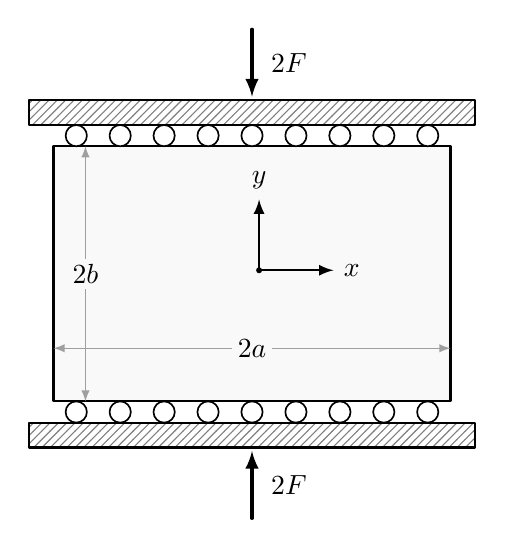
\begin{tikzpicture}[
  scale=0.9,
  line cap=round,
  line join=round
]
  % Specimen
  \draw[thick, fill=gray!5]
    (-2.8,-1.8) rectangle (2.8,1.8);

  % Rigid platens
  \draw[
    thick,
    pattern=north east lines,
    pattern color=gray
  ] (-3.15,2.10) rectangle (3.15,2.45);
  \draw[
    thick,
    pattern=north east lines,
    pattern color=gray
  ] (-3.15,-2.45) rectangle (3.15,-2.10);

  % Roller bearings
  \foreach \x in {
    -2.48,-1.86,-1.24,-0.62,0,
     0.62, 1.24, 1.86, 2.48
  } {
    \draw[semithick, fill=white] (\x, 1.95) circle (0.15);
    \draw[semithick, fill=white] (\x,-1.95) circle (0.15);
  }

  % Applied compressive loads
  \draw[-latex, very thick]
    (0,3.45) -- (0,2.50)
    node[midway, right=3pt] {$2F$};
  \draw[-latex, very thick]
    (0,-3.45) -- (0,-2.50)
    node[midway, right=3pt] {$2F$};

  % Specimen dimensions
  \draw[latex-latex, gray!75]
    (-2.8,-1.05) -- (2.8,-1.05)
    node[midway, fill=gray!5, inner sep=2pt, text=black] {$2a$};
  \draw[latex-latex, gray!75]
    (-2.35,-1.8) -- (-2.35,1.8)
    node[midway, fill=gray!5, inner sep=2pt, text=black] {$2b$};

  % Coordinate axes
  \fill (0.10,0.05) circle (1.2pt);
  \draw[-latex, thick]
    (0.10,0.05) -- (1.15,0.05)
    node[right] {$x$};
  \draw[-latex, thick]
    (0.10,0.05) -- (0.10,1.05)
    node[above] {$y$};
\end{tikzpicture}
\caption{Geometry and loading for the Mandel problem and the reacting Mandel problem.}
\label{fig:verification_setup}
\end{figure}

\subsection{Mandel problem}\label{sec:mandel}
%
The Mandel problem \cite{cheng1988direct} is a commonly used verification problem in poroelasticity that demonstrates the feedback between mechanical deformation and pore fluid pressure evolution in uniaxial compression of a plane strain poroelastic medium.  In what follows, we compare our full reacting mixture theory, i.e.\ \emph{mixture model}, with standard poromechanics formulations for infinitesimal strains, i.e.\ the Biot equations.

The geometry, roller loading, and dimensions used for this problem and for the reacting Mandel problem in \S~\ref{sec:mandel react} are shown in Fig.~\ref{fig:verification_setup}.
%
\begin{subequations}
\begin{align}
  \mathbf{0} &= \nabla_{\mathbf{x}} \cdot \left(\boldsymbol{\sigma}^{\prime\prime}_s - B \bar{p}_f \mathbf{I}\right), \label{eq:infa} \\
  0 &= B \mbox{tr}(\dot{\bs\varepsilon}) + \frac{1}{M} \frac{\partial \bar{p}_f}{\partial t} - \nabla_{\mathbf{x}} \cdot \left(\frac{\mathbf{k}}{\mu}\nabla_{\mathbf{x}} p\right), \label{eq:infb}
\end{align}
  \label{eq:infinitesimal_model}
\end{subequations}
%
where $\bs\sigma^{\prime\prime}_s$ is the effective Cauchy stress ($p$ held fixed) of the solid skeleton and $\dot{\bs\varepsilon}$ is the linearized strain rate tensor. $B = 1 - \nicefrac{K}{K_s}$ is the Biot coefficient where $K$ is the bulk modulus of the solid skeleton. The Biot modulus is
%
\begin{equation*}
M = \frac{K_s K_f}{K_f (B - \phi) + K_s \phi},
\end{equation*}
%
We call equations \eqref{eq:infinitesimal_model} the \emph{infinitesimal model}.

The classical approaches to poroelasticity use constitutive equations for the solid skeleton; however, our reacting mixture model uses constitutive equations for the individual minerals comprising the solid skeleton.  From the mixture rules derived in Appendix~\ref{sec:biot}, with a single solid phase ($\phi_B = 0$, no reactions) and porosity $\phi = 0.2$, the effective skeleton properties are $G_{\text{eff}} = (1-\phi) G_A = 0.8\, G_A$ and $K^\star_{\text{eff}} = K^\star_A$.  Using a shear modulus $G_A = 100$~MPa gives an effective shear modulus $G = 80$~MPa for the solid skeleton. We solve the Mandel problem with fluid properties set to water and initial pressure $\bar{p}_f(\mbf{X}_s, 0) = 0.5$.  The results are shown in Fig.~\ref{fig:mandel}, where good agreement among all fields is demonstrated.  It may be surprising that the infinitesimal and finite-deformation mixture models give similar results; this is due to the incompressible mineral solid, since the nonlinearity of the finite-deformation model under uniaxial compression is related to the compressibility. However, the limitations of the small-strain assumption become apparent as the applied top load increases. Fig.~\ref{fig:mandel_1e9} illustrates the pore pressure $(p_{avg})$ and displacements $(u_{x_{avg}}, u_{y_{avg}})$ across a range of top loads. As the load approaches $10^{10}$, the infinitesimal model deviates significantly from the proposed mixture model. The large deformation kinematics capture geometric nonlinearities that result in a stiffer macroscopic response, evidenced by reduced vertical compression and lateral expansion and a correspondingly higher average pore pressure buildup than predicted by the infinitesimal model.

\begin{figure}[htbp]
  \centering
  \begin{subfigure}[b]{0.50\textwidth} % Equalized width
    \centering
    % Replaced ! with a fixed height like 7.5cm
    \resizebox{\linewidth}{13cm}{\input{figs/1e8_mandel_comparison.pgf}}
    \caption{Top load $F=10^8$}
    \label{fig:mandel_1e8}
  \end{subfigure}\hfill
  \begin{subfigure}[b]{0.50\textwidth} % Equalized width
    \centering
    % Replaced ! with the exact same fixed height
    \resizebox{\linewidth}{13cm}{\input{figs/top_load_plot.pgf}}
    \caption{Effect of top load on pressure and displacements}
    \label{fig:mandel_1e9}
  \end{subfigure}
  \caption{Comparison of solutions to the Mandel problem.}
  \label{fig:mandel}
\end{figure}


\subsection{``Undrained'' reacting verification problem}\label{sec:undrained}

Recall equations~\eqref{eq:mass_all} except now we make the additional assumptions that the fluid density is also incompressible $\dot{\bar{\rho}}_f = 0$, and there is no relative motion between the fluid and solid, i.e.\ $\mbf{v}_f = \mbf{v}_s$. This corresponds to a porous medium where the individual pores are not connected and hence the pore fluid cannot flow relative to the solid. In this limit, the mass balances \eqref{eq:mass_all} become
%
\begin{subequations}
\begin{align}
  \dot{\phi}  + \phi \nabla_{\mathbf{x}} \cdot \mathbf{v}_s &= \frac{c^{+}_f}{\bar\rho_f}, \label{eq:mass_f_2} \\
  \dot{\phi}_A + \phi_A \nabla_{\mathbf{x}} \cdot \mathbf{v}_s &= \frac{c^{+}_A}{\bar\rho_A}, \label{eq:mass_A_2} \\
  \dot{\phi}_B + \phi_B \nabla_{\mathbf{x}} \cdot \mathbf{v}_s &= \frac{c^{+}_B}{\bar\rho_B}. \label{eq:mass_B_2}
\end{align}
  \label{eq:mass_all_2}
\end{subequations}
%
Summing these equations while substituting the constraints \eqref{eq:sum_phi} and \eqref{eq:sum_cplus} and recognizing $\dot{\phi} + \dot{\phi}_A + \dot{\phi}_B = 0$ we have
%
\begin{align}
  \nabla_{\mbf{x}} \cdot \mbf{v}_s &= \frac{c^{+}_A}{\bar{\rho}_A} + \frac{c^{+}_B}{\bar{\rho}_B} + \frac{c^{+}_f}{\bar{\rho}_f} \notag \\
  &= \frac{c^{+}_A}{\bar{\rho}_A} + \frac{c^{+}_B}{\bar{\rho}_B} - \frac{1}{\bar{\rho}_f}\left(c^{+}_A + c^{+}_B\right) \notag \\
  &= c^{+}_A\left(\frac{1}{\bar{\rho}_A} - \frac{1}{\bar{\rho}_f}\right) + c^{+}_B\left(\frac{1}{\bar{\rho}_B} - \frac{1}{\bar{\rho}_f}\right)
  \label{eq:overall_mass_2}
\end{align}
%
Recall the well-known identity $\dot{J}_s = J_s \nabla_{\mbf{x}} \cdot \mbf{v}_s$ and substitute this into \eqref{eq:mass_all_2} and \eqref{eq:overall_mass_2} while pulling all equations back to the reference configuration of the solid to obtain

%
\begin{subequations}
\begin{align}
  J_s \left.\p{\phi}{t}\right\vert_{\mbf{X}_s} + \phi \left.\p{J_s}{t}\right\vert_{\mbf{X}_s}   +\frac{\dot{c}_A}{\bar\rho_f} +\frac{\dot{c}_B}{\bar\rho_f} &= 0, \label{eq:mass_f_3} \\
  J_s \left.\p{\phi_A}{t}\right\vert_{\mbf{X}_s} + \phi_A \left.\p{J_s}{t}\right\vert_{\mbf{X}_s} - \frac{\dot{c}_A}{\bar\rho_A} &= 0, \label{eq:mass_A_3} \\
  J_s \left.\p{\phi_B}{t}\right\vert_{\mbf{X}_s} + \phi_B \left.\p{J_s}{t}\right\vert_{\mbf{X}_s}  - \frac{\dot{c}_B}{\bar\rho_B} &= 0, \label{eq:mass_B_3} \\
  \left.\p{J_s}{t}\right\vert_{\mbf{X}_s} - \dot{c}_A\left(\frac{1}{\bar{\rho}_A} - \frac{1}{\bar{\rho}_f}\right) - \dot{c}_B\left(\frac{1}{\bar{\rho}_B} - \frac{1}{\bar{\rho}_f} \right) &= 0
\end{align}
\end{subequations}
%
which are coupled nonlinear ordinary differential equations that can be solved for the evolution of the volume fractions and $J_s$ numerically.  Using the previously introduced definition of Lagrangian volume fractions, i.e.\ $\Phi_\xi = J_s \phi_\xi$ we can see that the first two terms in \eqref{eq:mass_f_3}--\eqref{eq:mass_B_3} can be rewritten and the equations rearranged to yield
%
\begin{subequations}
\begin{align}
  \left.\p{\Phi}{t}\right\vert_{\mbf{X}_s} &= -\frac{\dot{c}_A}{\bar\rho_f} - \frac{\dot{c}_B}{\bar\rho_f}, \label{eq:mass_f_3a} \\
  \left.\p{\Phi_A}{t}\right\vert_{\mbf{X}_s} &= \frac{\dot{c}_A}{\bar\rho_A}, \label{eq:mass_A_3a} \\
  \left.\p{\Phi_B}{t}\right\vert_{\mbf{X}_s} &= \frac{\dot{c}_B}{\bar\rho_B}, \label{eq:mass_B_3a} \\
  \left.\p{J_s}{t}\right\vert_{\mbf{X}_s} &=  \dot{c}_A\left(\frac{1}{\bar{\rho}_A} - \frac{1}{\bar{\rho}_f}\right) + \dot{c}_B\left(\frac{1}{\bar{\rho}_B} - \frac{1}{\bar{\rho}_f} \right), \label{eq:mass_J_3a}
\end{align}
  \label{eq:mass_3aa}
\end{subequations}
%
If $\dot{c}_{A}$ and $\dot{c}_{B}$ are independent of the $\Phi_\xi$, e.g.\ $\dot{c}_{A} = \text{constant}$ and $\dot{c}_{B} = \text{constant}$, then equations \eqref{eq:mass_3aa} have the analytic solutions
%
\begin{subequations}
\begin{align}
  \Phi(t) &= \phi_0 - \left(\frac{\dot{c}_A}{\bar\rho_f} + \frac{\dot{c}_B}{\bar\rho_f}\right) t, \label{eq:mass_f_3a_sol} \\
  \Phi_A(t) &= \phi_{A0} + \frac{\dot{c}_A}{\bar\rho_A} t, \label{eq:mass_A_3a_sol} \\
  \Phi_B(t) &= \phi_{B0} + \frac{\dot{c}_B}{\bar\rho_B} t, \label{eq:mass_B_3a_sol} \\
  J_s &=  1 + \dot{c}_A\left(\frac{1}{\bar{\rho}_A} - \frac{1}{\bar{\rho}_f}\right)t + \dot{c}_B\left(\frac{1}{\bar{\rho}_B} - \frac{1}{\bar{\rho}_f} \right) t, \label{eq:mass_J_3a_sol}
\end{align}
\end{subequations}
%
where $J_s(t=0) = 1$. Combining the solutions \eqref{eq:mass_f_3a_sol}--\eqref{eq:mass_B_3a_sol} with \eqref{eq:mass_J_3a_sol} and the definition of the Lagrangian volume fractions allows one to reconstruct the evolution of the volume fractions $\phi_\xi$. We call this the \emph{ODE model}. We can mimic the behavior of the ODE model in our full reacting mixture model by setting the fluid bulk modulus $K_f$ to a very high value to approximate fluid incompressibility and setting no-flow boundaries on all sides so that no new fluid enters the system and pressure gradients do not arise to cause fluid motion with respect to solid skeleton.  The results of these verification simulations are shown in Fig.~\ref{fig:swiss_cheese}a and demonstrate good agreement between the two models. As the reaction proceeds the domain contracts, $J_s<1$, because the overall volume shrinks during the reaction. It is important to note that the solid volume increases, but it is compensated by the shrinking of the porosity. During this reaction the fluid pressure drops, which induces suction that leads to contraction.

\subsection{``Drained'' reacting verification problem}\label{sec:drained}

Once again recall equations~\eqref{eq:mass_all} with the additional assumption that the fluid density is incompressible $\dot{\bar{\rho}}_f = 0$; however, now assume there is constant fluid pressure on all boundaries equal to the initial pore pressure, no reactions occur on the boundary (only in the pore space), and there is sufficient permeability such that fluid flows freely into the system to replace fluid lost to reactions and gradients in fluid pressure remain negligible.  In this case, there will be no volume change of the solid skeleton, i.e.\ $\nabla_{\mbf{x}} \cdot \mbf{v}_s = 0$ or $J_s(t) = 1$ and the equations become
%
\begin{subequations}
\begin{align}
  \dot{\phi}  + \phi \nabla_{\mathbf{x}} \cdot \mathbf{v}_f &= \frac{c^{+}_f}{\bar\rho_f}, \label{eq:mass_f_4} \\
  \dot{\phi}_A  &= \frac{\dot{c}_A}{\bar\rho_A}, \notag \\
  \dot{\phi}_B  &= \frac{\dot{c}_B}{\bar\rho_B}. \notag
\end{align}
\end{subequations}
%
Summing these equations while substituting the constraint \eqref{eq:sum_cplus} and $\dot{\phi} + \dot{\phi}_A + \dot{\phi}_B = 0$ we have
%
\begin{align}
  \nabla_{\mbf{x}} \cdot \mbf{v}_f &= \frac{1}{\phi}\left(\frac{\dot{c}_A}{\bar{\rho}_A} + \frac{\dot{c}_B}{\bar{\rho}_B} + \frac{c^{+}_f}{\bar{\rho}_f}\right).
  \label{eq:overall_mass_4aaa}
\end{align}
%
Substituting \eqref{eq:overall_mass_4aaa} into \eqref{eq:mass_f_4} gives the final system of equations in the current configuration
%
\begin{subequations}
\begin{align}
  \dot{\phi}   &= -\frac{\dot{c}_A}{\bar\rho_A} - \frac{\dot{c}_B}{\bar\rho_B}, \notag \\
  \dot{\phi}_A  &= \frac{\dot{c}_A}{\bar\rho_A}, \notag \\
  \dot{\phi}_B  &= \frac{\dot{c}_B}{\bar\rho_B}. \notag
\end{align}
\end{subequations}
%

If $\dot{c}_{A}$ and $\dot{c}_{B}$ are independent of the $\phi_\xi$, e.g.\ $\dot{c}_{A} = \text{constant}$ and $\dot{c}_{B} = \text{constant}$, then this system of equations has the analytic solution
%
\begin{subequations}
\begin{align}
  \phi(t)   &= \phi_0 - \left(\frac{\dot{c}_A}{\bar\rho_A} + \frac{\dot{c}_B}{\bar\rho_B}\right) t, \notag \\
  \phi_A(t) &= \phi_{A0} + \frac{\dot{c}_A}{\bar\rho_A} t, \notag \\
  \phi_B(t) &= \phi_{B0} + \frac{\dot{c}_B}{\bar\rho_B} t. \notag
\end{align}
\end{subequations}

Comparison between the drained ODE solution and the MOOSE implementation of our reacting mixture theory is shown in Fig.~\ref{fig:swiss_cheese}b and demonstrates good agreement.

\begin{figure}[htbp]
  \centering
  \begin{subfigure}[t]{0.48\textwidth}
    \vspace{0pt}
    \centering
    \resizebox{\linewidth}{!}{\input{figs/CaseA_linear_panel_plot.pgf}}
    \caption{``Undrained'' Reacting Verification Problem}
  \end{subfigure}
  \hfill
  \begin{subfigure}[t]{0.48\textwidth}
    \vspace{0pt}
    \centering
    \resizebox{\linewidth}{!}{\input{figs/CaseB_linear_panel_plot.pgf}}
    \caption{``Drained'' Reacting Verification Problem}
  \end{subfigure}
  \caption{Comparison between analytic ODE solutions to the full reacting mixture formulation implemented in the finite element framework MOOSE \cite{harbour2025moose}.}
\label{fig:swiss_cheese}
\end{figure}
This problem illustrates one of the advantages of the distention formulation, namely that reaction products can simply fill the pores without inducing deformation of the skeleton. Comparing undrained and drained cases, we see that porosity is exhausted in Fig.~\ref{fig:swiss_cheese}a but not in Fig.~\ref{fig:swiss_cheese}b, although both start with the same porosity. This is due to the influx of additional water in the drained case, where the reaction stops once reactant is exhausted.

\subsection{Transient Volumetric Response}\label{sec:transient}
Now we consider a problem that combines the two responses we have seen above in \S~\ref{sec:undrained} and \S~\ref{sec:drained}. We use an open (drained) system but with a permeability sufficiently low that reactions consume fluid faster than it can be replaced. This leads to an initial contraction similar to the undrained case in \S~\ref{sec:undrained}, followed by an expansion as the pore fluid pressure equilibrates diffusively. For this comparison, the problem is constrained such that deformation can only occur in the horizontal direction and the top, bottom, and left side boundaries have no-flow conditions.  The right boundary is fixed at the initial fluid pressure ($\bar{p}_f = 0$ in this case).

\begin{figure}[htbp]
    \centering
    \resizebox{0.7\textwidth}{!}{\input{figs/jacobian_transient_all_cases_log.pgf}}
    \caption{Comparison of transient cases on a logarithmic scale.}
    \label{fig:jacobian_transient}
\end{figure}

Fig.~\ref{fig:jacobian_transient} shows the change in the solid skeleton Jacobian ($J_s$) over time for different values of the permeability, which has been assumed, without loss of generality, to remain constant in each simulation.  The reaction consumes pore fluid, inducing a localized pore pressure drop. In the transient cases, this pressure deficit causes the solid skeleton to initially compress ($J < 1$). As fluid diffuses into the system from the boundary to replace the consumed mass, the pressure recovers, and the skeleton elastically rebounds to its initial volume ($J \to 1$). Lower permeabilities ($k = 10^{-16}$ and $10^{-17}$~m$^2$) naturally delay this recovery.  For all cases, the undrained solution from \S~\ref{sec:undrained} provides a lower asymptote. In the purely undrained case, fluid cannot be replenished, resulting in a permanent volume reduction.
%
\begin{figure}[htbp]
    \centering
    \begin{tikzpicture}
        \node[anchor=south west, inner sep=0] (image) at (0,0) {\includegraphics[width=0.95\textwidth]{figs/bar_animation.png}};
        \begin{scope}[x={(image.south east)},y={(image.north west)}]
            \node[anchor=east, font=\large] at (0.08, 0.92) {$t = 0 s$};
            \node[anchor=east, font=\large] at (0.08, 0.74) {$t = 10 s$};
            \node[anchor=east, font=\large] at (0.08, 0.57) {$t = 110 s$};
            \node[anchor=east, font=\large] at (0.08, 0.40) {$t = 800 s$};
            \node[anchor=east, font=\large] at (0.08, 0.24) {$t = 5000 s$};
        \end{scope}
    \end{tikzpicture}
    \caption{Dynamic volumetric response to internal pressure variations over time ($t$) for the $k = 10^{-17}$~m$^2$ case.}
    \label{fig:bar_animation}
\end{figure}

Fig.~\ref{fig:bar_animation} illustrates the spatial distribution of pressure and the resulting volume changes at discrete time intervals for the $k = 10^{-17}$~m$^2$ case. At time ($t=0$ s), the initial state is changed by the fluid consuming reactions, generating a transient negative pressure gradient (observed from $t=10$ s to $110$ s). This pressure gradient drives significant volume reduction. As fluid flows in through the boundary over time ($t = 800$ s), the pressure gradient gradually dissipates, allowing the domain to expand until it achieves its original volume ($t = 5000$ s).

\subsection{Reacting Mandel problem}\label{sec:mandel react}

Finally, we illustrate the effect of the evolving mechanical properties of the solid skeleton as the reaction progresses during mechanical deformation. We simulate a reacting Mandel problem, set up as in \S~\ref{sec:mandel}, but where the solid skeleton undergoes a hydration reaction. The simulation starts with an anhydrite volume fraction $\phi_A = 0.559$ and an initial porosity $\phi = 0.441$. The domain is subjected to an applied top traction of $1 \times 10^{8}$~Pa. We assign a high permeability of $k = 1 \times 10^{-5}$~m$^2$ and a reaction rate constant of $100$~s$^{-1}$.

As the reaction progresses, anhydrite and pore fluid are consumed to precipitate gypsum. At the completion of the reaction, the gypsum volume fraction reaches $\phi_G = 0.91$. Consequently, the remaining porosity is reduced to $\phi = 0.09$. 

In the standard incompressible Mandel problem, discussed in \S~\ref{sec:mandel}, the displacements are instantaneous and do not evolve in time, as shown in Fig.~\ref{fig:mandel}a. However, due to the large difference in mechanical properties, these static displacements are larger for gypsum than for anhydrite. In contrast, the displacements of the reacting Mandel problem evolve in time as shown in Fig.~\ref{fig:reacting_mandel_spatial}. The instantaneous displacement upon loading is that of pure anhydrite. Over time, as the reaction proceeds, the displacements become larger and asymptote to the displacements of pure gypsum. This softening of the material is a characteristic of many hydration reactions that is often neglected and may limit buildup of stresses that induce fracturing.


\begin{figure}[htbp]
    \centering
    \resizebox{0.7\textwidth}{!}{\input{figs/reacting_mandel_spatial.pgf}}
    \caption{Horizontal ($u_x$) and vertical ($u_y$) displacements in the reacting Mandel problem. The color gradient indicates the change in displacements with time on a logarithmic scale from $10^{-4}$ to $10^{4}$ seconds. Markers distinguish the baseline unreacted anhydrite response from the fully reacted gypsum response.}
    \label{fig:reacting_mandel_spatial}
\end{figure}


\section{Conclusions}

We have presented a finite-deformation formulation for a reacting fully saturated three-phase porous mixture built on Bedford and Drumheller's mixture theory \cite{drumheller1980thermomechanical} and the distention gradient concept of Drumheller \cite{drumheller2000}.  A key idea is a multiplicative decomposition of the deformation gradient into distention and true deformation.  We show that, for incompressible solid phases, this reduces kinematically to the classical volumetric--isochoric multiplicative split.  We nevertheless retain the distention concept because it motivates a decomposition of the free energy into isochoric and distention components and provides a straightforward path to future extensions with compressible solid phases for which $J_s \neq \alpha_s$.  This allows the model to distinguish between reaction-induced volume changes that fill pore space and those that strain the skeleton---a distinction that eigenstrain-based models cannot make.

The Coleman--Noll procedure applied to a $\phi$-dependent distention energy yields two quantities absent from standard poromechanics: a modified porosity-conjugate pressure $\bar{p}^\star_\xi$ that includes a porosity-correction factor $(1 + \frac{1}{2}\ln J_s)$, and a porosity-conjugate pressure $p^\star_\phi$ that enters the momentum balance as an additional body force.  Both corrections are $O(\varepsilon^2)$ at small strains, so the theory reduces exactly to Biot poromechanics with $B = 1$ in the appropriate limit.  The effective elastic properties of the skeleton update automatically through mixture rules as the reaction progresses, which is important for reactions like serpentinization where the reactant and product have substantially different elastic moduli.

A generalized Darcy-like relative flux accounts for fluid consumption by reactions, and a Lagrange multiplier $\tau$---we call the \emph{exchange potential}---evolves as a generalized chemical potential whose gradient drives chemically induced fluid transport.  All governing equations have been pulled back to the reference configuration and cast in weak form suitable for finite element implementation.  Verification against the Mandel problem solution and simplified ODE models for undrained and drained reacting systems demonstrates that the implementation is consistent with the theory.

The present formulation assumes incompressible solid phases, which limits the Biot coefficient to $B = 1$.  For geological materials with non-negligible grain compressibility, the distention framework retained here provides a natural path to relaxing this assumption by allowing $\alpha_s$ to evolve independently of $J_s$.  Future work will apply the theory to spatially coupled reacting systems, including serpentinization of peridotite, and explore coupling with fracture models for prediction of reaction-induced fracturing.

\section{Acknowledgements}
The first author with like to thank Prof. D.~Nicolas Espinoza for helpful conversations that inspired this work. This work was funded by the U.S. Department of Energy under awards DE-FE0032349 ``Hydrogen Storage in Salt Caverns in the Permian Basin: Seal Integrity Evaluation and Field Test'' and DE-AR0001864283 assigned
control number 2784-1755 ``Cyclic Injection for Commercial Seismic-Safe Geologic H2 Production.''
\appendix
\section{Variational Derivation}
\label{sec:variational}

We derive the governing equations from Hamilton's extended principle, following Bedford \& Drumheller~\cite{drumheller1980thermomechanical} and Drumheller~\cite{drumheller2000}, adapted to a fully saturated system with porosity-dependent solid free energies.

Each phase has volume fraction~$\phi_\xi$, intrinsic density~$\bar\rho_\xi$, partial density $\rho_\xi = \phi_\xi\bar\rho_\xi$, velocity~$\mbf{v}_\xi$, deformation gradient~$\mbf{F}_\xi$, and Jacobian $J_\xi = \det(\mbf{F}_\xi)$.  The solid phases share a common trajectory ($\mbf{v}_A = \mbf{v}_B = \mbf{v}_s$, $\mbf{F}_A = \mbf{F}_B = \mbf{F}_s$, $J_A = J_B = J_s$).  The porosity is $\phi = \phi_f$ (i.e.\ fully saturated \eqref{eq:sum_phi}).  The mass added per unit reference volume to phase~$\xi$ by reactions is~$c_\xi$, with rate per unit current volume $c^+_\xi = \dot{c}_\xi / J_\xi$.

The free energies of the solid phases are written as $\psi_A(\mbf{F}_s, \phi)$ and $\psi_B(\mbf{F}_s, \phi)$, retaining the full deformation gradient and the current porosity as independent arguments.  The multiplicative decomposition $\mbf{F}_s = \mbf{A}_s \mbf{\bar F}_s$ is \emph{not} imposed at this stage; it enters later in the Coleman--Noll procedure (Appendix~\ref{sec:coleman}) when a specific constitutive form is adopted.

\subsection{Variational principle and its terms}

The extended Hamilton's principle is
\begin{equation*}
  \int_{t_1}^{t_2}\left[\delta(T - U) + \delta W + \sum_k \delta C_k\right] dt = 0,
\end{equation*}
with kinetic energy, internal energy, virtual work, and three constraint functionals.
\begin{align*}
  T &= \sum_\xi \int_{\mc{B}} \tfrac{1}{2}\rho_\xi\,\mbf{v}_\xi\cdot\mbf{v}_\xi \dv,  \\[4pt]
  U &= \sum_\xi \int_{\mc{B}_{\xi 0}} \rho_{\xi 0}\,\psi_\xi \,dV_\xi,  \\[4pt]
  \delta W &= \sum_\xi \int_{\mc{B}} \left[(\rho_\xi\mbf{g} + \mbf{b}_\xi)\cdot\delta\mbf{x}_\xi + \mc{L}_\xi\,\frac{\delta c_\xi}{J_\xi}\right] \dv,  \\[4pt]
  C_1 &= \int_{\mc{B}} \lambda\left(\sum_\xi\phi_\xi - 1\right) \dv,  \\[4pt]
  C_2 &= \sum_\xi \int_{\mc{B}_{\xi 0}} \mu_\xi\left(J_\xi - \frac{\phi_{\xi 0}\bar\rho_{\xi 0} + c_\xi}{\phi_\xi\bar\rho_\xi}\right) dV_\xi,  \\[4pt]
  C_3 &= \int_{\mc{B}} \tau\sum_\xi c^+_\xi \dv.
\end{align*}
The Helmholtz free energies are $\psi_A(\mbf{F}_s, \phi)$, $\psi_B(\mbf{F}_s, \phi)$, $\psi_f(\bar\rho_f)$.  The interaction forces satisfy \eqref{eq:sum_b}, and $\mc{L}_\xi$ is a generalized force conjugate to mass transfer (identified later via Coleman--Noll).  The Lagrange multipliers~$\lambda$, $\mu_\xi$, and~$\tau$ enforce the volume fraction constraint, the phase material mass balances including mass transfer, and the mixture mass balance \eqref{eq:sum_cplus}, respectively.

Most of the required variations are detailed in Bedford \& Drumheller~\cite{drumheller1980thermomechanical} and will be omitted here; however, there are some new terms in this work that are derived below.

\subsection{Variation of the internal energy}

The internal energy is
\[
  U = \int_{\mc{B}_{s0}} \left[\rho_{A0}\,\psi_A(\mbf{F}_s, \phi) + \rho_{B0}\,\psi_B(\mbf{F}_s, \phi)\right] dV_s + \int_{\mc{B}_{f0}} \rho_{f0}\,\psi_f(\bar\rho_f)\,dV_f.
\]
Since the solid reference integrals are over the fixed reference domain~$\mc{B}_{0}$, the variation acts only on the integrand.  The solid contribution is
\begin{align}
  \delta U_s &= \int_{\mc{B}_{s0}} \sum_{\xi=A,B} \rho_{\xi 0} \left[\left.\p{\psi_\xi}{F_{kl}}\right\vert_\phi \delta F_{kl} + \left.\p{\psi_\xi}{\phi}\right\vert_{\mbf{F}_s} \delta\phi \right] dV_s.
  \label{eq:deltaU_solid}
\end{align}

The variation $\delta F_{kl} = \partial(\delta x_{s,k})/\partial X_{s,l}$ produces the standard stress divergence upon integration by parts.  Transforming to the current configuration gives
\begin{equation*}
  \int_{\mc{B}_{0}} \rho_{\xi 0}\,\left.\p{\psi_\xi}{F_{kl}}\right\vert_\phi \delta F_{kl}\, dV_s = -\int_{\mc{B}} \nabla_{\mbf{x}} \cdot \bs\sigma'_\xi \cdot \delta\mbf{x}_s \dv + \text{boundary terms},
\end{equation*}
where the effective Cauchy stress is defined through
\begin{equation*}
  \bs\sigma'_\xi = \frac{1}{J_s} \rho_{\xi 0}\,\p{\psi_\xi}{\mbf{F}_s}\bigg\vert_\phi\, \mbf{F}_s^T.
\end{equation*}
The notation $|_\phi$ emphasizes that this derivative is taken at fixed porosity.

\subsection{Porosity variation via the inter-phase identity}

The porosity~$\phi = \phi_f$ is a spatial field naturally associated with the fluid phase, yet it appears as an argument of the solid free energies $\psi_\xi(\mbf{F}_s, \phi)$ in the integral over the solid reference configuration.  Since this integral is taken at fixed~$\mbf{X}_s$, we require the variation of~$\phi$ at fixed~$\mbf{X}_s$.  Because $\phi$ is a fluid field, we use the inter-phase variation identity (equation~(1.26) of Bedford \& Drumheller~\cite{bedford1983theories})
\begin{equation}
  \left.\delta\Gamma_{\zeta}\right|_{\mbf{X}_{\xi}} = \delta\Gamma_{\zeta} - \nabla_{\mbf{x}}\Gamma_{\zeta} \cdot \left(\delta\mbf{x}_{\zeta} - \delta\mbf{x}_{\xi}\right),
  \label{eq:BD_identity}
\end{equation}
which relates the variation of a field~$\Gamma$ belonging to phase~$\zeta$, evaluated at the reference position of phase~$\xi$, to the material variation of~$\Gamma$ following~$\zeta$ plus a correction for the relative displacement.  Setting $\Gamma = \phi$, $\zeta = f$, $\xi = s$,
\begin{equation}
  \left.\delta\phi\right|_{\mbf{X}_s} = \delta\phi_f - \nabla_{\mbf{x}}\phi \cdot \left(\delta\mbf{x}_f - \delta\mbf{x}_s\right),
  \label{eq:delta_phi}
\end{equation}
where $\delta\phi_f \equiv \left.\delta\phi\right|_{\mbf{X}_f}$ is the material variation of~$\phi$ following the fluid.

Defining
\begin{equation*}
  p^\star_\phi \equiv \sum_{\xi=A,B} \rho_\xi\,\left.\p{\psi_\xi}{\phi}\right\vert_{\mbf{F}_s},
\end{equation*}
and substituting~\eqref{eq:delta_phi} into~\eqref{eq:deltaU_solid}, the porosity-dependent part of the solid energy variation becomes
\begin{align}
  \int_{\mc{B}_{0}} \sum_{\xi=A,B} \rho_{\xi 0}\,\left.\p{\psi_\xi}{\phi}\right\vert_{\mbf{F}_s}\, \left.\delta\phi\right|_{\mbf{X}_s}\, dV_s
  &= \int_{\mc{B}} p^\star_\phi\, \delta\phi_f \dv
  - \int_{\mc{B}} p^\star_\phi\, \nabla_{\mbf{x}}\phi \cdot \delta\mbf{x}_f \dv
  + \int_{\mc{B}} p^\star_\phi\, \nabla_{\mbf{x}}\phi \cdot \delta\mbf{x}_s \dv.
  \label{eq:phi_variation_split}
\end{align}
The three terms have distinct roles: (i)~$p^\star_\phi\,\delta\phi_f$ contributes to the coefficient of $\delta\phi_f$; (ii)~$-p^\star_\phi\,\nabla_{\mbf{x}}\phi \cdot \delta\mbf{x}_f$ is a body force on the \emph{fluid}; (iii)~$+p^\star_\phi\,\nabla_{\mbf{x}}\phi \cdot \delta\mbf{x}_s$ is a body force on the \emph{solid}.  The $\nabla_{\mbf{x}}\phi$ body forces on the solid and fluid are equal and opposite by construction.

The variation of the fluid internal energy follows the standard procedure detailed in Bedford \& Drumheller~\cite{drumheller1980thermomechanical} and is absorbed into the collected variational principle below.

\subsection{Collected variational principle}

Evaluating all variations and collecting by independent variations $\delta\mbf{x}_\xi$, $\delta\phi_\xi$, $\delta\bar\rho_\xi$, $\delta c_\xi$,
\begin{align}
  0 = \sum_\xi \int_{\mc{B}} \bigg\{
  &\bigg[-\rho_\xi\mbf{a}_\xi + \nabla_{\mbf{x}}\cdot \bs\sigma'_\xi + \rho_\xi\mbf{g} + \mbf{b}_\xi
  - \nabla_{\mbf{x}}\left(\mu_\xi J_\xi\right) + \lambda\nabla_{\mbf{x}}\phi_\xi + c^+_\xi\nabla_{\mbf{x}}\tau
  \bigg]\cdot\delta\mbf{x}_\xi \notag \\[4pt]
  &+ \bigg[\frac{\mu_\xi J_\xi}{\phi_\xi} - \lambda\bigg]\,\delta\phi_\xi
  + \bigg[\frac{\mu_\xi J_\xi}{\bar\rho_\xi} - \rho_\xi\p{\psi_\xi}{\bar\rho_\xi}\bigg]\,\delta\bar\rho_\xi \notag \\[4pt]
  &+ \bigg[\frac{1}{2}\mbf{v}_\xi\cdot\mbf{v}_\xi + \mc{L}_\xi - \frac{D_\xi\tau}{Dt} - \frac{\mu_\xi J_\xi}{\rho_\xi}\bigg]\frac{\delta c_\xi}{J_\xi}
  \bigg\} \dv \notag \\[6pt]
  &+ \int_{\mc{B}} p^\star_\phi\, \delta\phi_f \dv
  + \int_{\mc{B}} p^\star_\phi\, \nabla_{\mbf{x}}\phi \cdot \delta\mbf{x}_s \dv
  - \int_{\mc{B}} p^\star_\phi\, \nabla_{\mbf{x}}\phi \cdot \delta\mbf{x}_f \dv.
  \label{eq:collected}
\end{align}
The last line contains the three specialized contributions from the porosity-dependent solid energy via~\eqref{eq:phi_variation_split}.

\subsection{Euler--Lagrange equations}

Since the variations are treated as independent and arbitrary, each coefficient in~\eqref{eq:collected} must vanish.  The coefficients of these variations are known as the Euler--Lagrange equations.

\paragraph{Pressure identifications.}  From the coefficient of $\delta\bar\rho_f$, and recognizing $\bar{p}_f$ as the thermodynamic fluid pressure identified through the Coleman-Noll procedure (Appendix~\ref{sec:coleman})
%
\begin{equation*}
  \bar{p}_f \equiv \bar{\rho}_f^2\frac{\,\partial\psi_f}{\partial\bar\rho_f},
\end{equation*}
%
giving $\mu_f J_f / \phi_f = \bar{p}_f$.  From $\delta\phi_\xi$ for the solid phases, $\mu_\xi J_s / \phi_\xi = \lambda$.  From $\delta\phi_f$, including the $p^\star_\phi$ contribution,
\begin{equation}
  \boxed{\lambda = \bar{p}_f + p^\star_\phi,}
  \label{eq:lambda_full}
\end{equation}
The Lagrange multiplier~$\lambda$ is \emph{not} simply the pore pressure when the solid energy depends on~$\phi$.

\paragraph{Fluid momentum.}  From the coefficient of $\delta\mbf{x}_f$, including the $-p^\star_\phi\,\nabla_{\mbf{x}}\phi$ body force from~\eqref{eq:phi_variation_split},
\begin{equation*}
  \rho_f\mbf{a}_f = \rho_f\mbf{g} + \mbf{b}_f - \nabla_{\mbf{x}}(\mu_f J_f) + \lambda\nabla_{\mbf{x}}\phi_f - p^\star_\phi\,\nabla_{\mbf{x}}\phi + c^+_f\nabla_{\mbf{x}}\tau.
\end{equation*}
Using $\mu_f J_f = \phi_f \bar{p}_f$ and $\lambda - \bar{p}_f = p^\star_\phi$,
\begin{align*}
  -\nabla_{\mbf{x}}(\phi_f \bar{p}_f) + \lambda\nabla_{\mbf{x}}\phi_f - p^\star_\phi\,\nabla_{\mbf{x}}\phi
  &= -\phi\nabla_{\mbf{x}}\bar{p}_f + p^\star_\phi\,\nabla_{\mbf{x}}\phi - p^\star_\phi\,\nabla_{\mbf{x}}\phi \\
  &= -\phi\nabla_{\mbf{x}}\bar{p}_f.
\end{align*}
The $p^\star_\phi\,\nabla_{\mbf{x}}\phi$ from the Lagrange multiplier algebra is exactly canceled by the direct body force from the inter-phase identity.  The fluid momentum balance is therefore
\begin{equation*}
  \boxed{\rho_f\mbf{a}_f = \rho_f\mbf{g} + \mbf{b}_f - \phi\nabla_{\mbf{x}}\bar{p}_f + c^+_f\left(\nabla_{\mbf{x}}\tau - \mbf{v}_f\right),}
\end{equation*}
which takes the same form as Bedford and Drumheller~\cite{drumheller1980thermomechanical} for the fluid phase.

\paragraph{Solid momentum.}  Summing over $\xi = A, B$ and including the $+p^\star_\phi\,\nabla_{\mbf{x}}\phi$ body force, using $\mu_\xi J_s = \phi_\xi\lambda$ and $\phi_A + \phi_B = 1-\phi$,
\begin{align*}
  -(1-\phi)\nabla_{\mbf{x}}\lambda + p^\star_\phi\,\nabla_{\mbf{x}}\phi
  &= -(1-\phi)\nabla_{\mbf{x}}\bar{p}_f - \nabla_{\mbf{x}}[(1-\phi)p^\star_\phi].
\end{align*}
The solid momentum balance becomes
\begin{equation*}
  \rho_s\mbf{a}_s = \nabla_{\mbf{x}}\cdot \bs\sigma'_s + \rho_s\mbf{g} - \mbf{b}_f - (1-\phi)\nabla_{\mbf{x}}\bar{p}_f - \nabla_{\mbf{x}}[(1-\phi)p^\star_\phi] - c^+_f\left(\nabla_{\mbf{x}}\tau - \mbf{v}_s\right).
\end{equation*}

\paragraph{Overall momentum.}  Summing solid and fluid balances, the $p^\star_\phi\,\nabla_{\mbf{x}}\phi$ body forces have already canceled within each phase balance,
\begin{equation}
  \boxed{\rho\mbf{a} = \nabla_{\mbf{x}}\cdot \bs\sigma'_s - \nabla_{\mbf{x}}\bar{p}_f - \nabla_{\mbf{x}}\left[(1-\phi)p^\star_\phi\right] + \rho\mbf{g} - c^+_f\left(\mbf{v}_f - \mbf{v}_s\right).}
  \label{eq:var_mom_overall}
\end{equation}
When $\psi_\xi$ does not depend on $\phi$ ($p^\star_\phi = 0$), this reduces to the standard form.  The cancellation of the $\nabla\phi$ body forces is guaranteed by the inter-phase identity~\eqref{eq:BD_identity}.

\paragraph{Evolution of $\tau$.}  From the coefficient of $\delta c_\xi$ and choosing to evaluate the functions for the reactant $A$
%
\begin{equation}
  \boxed{\left.\p{\tau}{t}\right|_{\mbf{X}_s} = \frac{1}{2}\mbf{v}_s\cdot\mbf{v}_s + \mathcal{L}_A - \frac{\lambda}{\bar\rho_A}.}
  \label{eq:var_tau_final}
\end{equation}

\subsection{Connection to the Coleman--Noll procedure}
\label{sec:coleman_connection}

The variational derivation and the Coleman--Noll procedure are complementary.  Hamilton's principle takes the free energies (e.g.\ $\psi_\xi(\mbf{F}_s, \phi)$) as functions of \emph{independent fields} (subject to constraints) and derives the momentum balances, pressure identifications, and body forces as Euler--Lagrange equations.  The Coleman--Noll procedure (Appendix~\ref{sec:coleman}) starts from the entropy inequality with the \emph{same} energy and derives constitutive restrictions.  The multiplicative decomposition $\mbf{F}_s = \mbf{A}_s \bar{\mbf{F}}_s$ is a constitutive choice imposed within the Coleman--Noll procedure, giving $\psi_\xi(\mbf{F}_s, \phi) = \psi^{\text{iso}}_\xi(\bar{\mbf{F}}_s) + \psi^{\text{dis}}_\xi(J_s, \phi)$, which is a specialization of the general $\psi_\xi(\mbf{F}_s, \phi)$ used in the variational principle.


\section{Coleman-Noll Procedure}
\label{sec:coleman}

The Coleman-Noll procedure is a systematic thermodynamic approach used to derive restrictions on constitutive models by ensuring compliance with the second law of thermodynamics. This procedure involves formulating the entropy inequality and identifying constraints that must be satisfied by any admissible constitutive relation. We apply this method to our reacting mixture to establish thermodynamically consistent constitutive equations.

We introduce the Helmholtz free energy $\psi_\xi$, the entropy $s_\xi$, and the temperature $\theta_\xi$ for each phase $\xi$. These quantities are related to the internal energy through the Legendre transformation
%
\begin{equation}
  E_\xi = \psi_\xi + s_\xi \theta_{\xi}.
  \label{eq:legendre}
\end{equation}
%
From \cite{drumheller2000}, the conservation of energy for phase $\xi$ in the mixture takes the form
\begin{equation}
  \rho_{\xi} \dot{E}_{\xi} + c_{\xi}^{+} E_{\xi} = \mathrm{tr}\left(\bs{\sigma}^{\prime}_{\xi} \mathbf{L}_{\xi}\right) + \phi_{\xi}\bar{p}_\xi  \frac{\dot{\bar\rho}_{\xi}}{\bar\rho_{\xi}} - \mathcal{L}_{\xi} c_{\xi}^{+} - \nabla_{\mathbf{x}} \cdot \mathbf{q}_{\xi} + \rho_{\xi} r_{\xi} + \dot{e}_{\xi},
  \label{eq:coe}
\end{equation}
%
where the terms on the right-hand side represent mechanical power, work due to density changes, latent heat of reaction, heat conduction, heat supply, and interaction energy, respectively. $\mathcal{L}_\xi$ is a generalized force that does work when $c^{+}_\xi$ changes.  Substituting the Legendre transformation \eqref{eq:legendre} into the energy equation \eqref{eq:coe} and rearranging to solve for the heat supply term $\rho_\xi r_{\xi}$ yields
%
\begin{align}
  \rho_{\xi} r_{\xi} =& \, \rho_{\xi} \dot{\psi}_{\xi} + \rho_\xi \dot{s}_\xi \theta_\xi + \rho_\xi s_\xi \dot\theta_\xi + c_{\xi}^{+} \left(\psi_{\xi} + s_\xi \theta_\xi\right) - \notag \\
  & \, \mathrm{tr}(\boldsymbol{\sigma}^{\prime T}_{\xi} \mathbf{L}_{\xi}) - \phi_{\xi} \bar{p}_\xi \frac{\dot{\bar\rho}_{\xi}}{\bar\rho_{\xi}} + \mathcal{L}_{\xi} c_{\xi}^{+} + \nabla_{\mathbf{x}} \cdot \mathbf{q}_{\xi} - \dot{e}_{\xi}, \label{eq:rho_r}
\end{align}
%
The second law of thermodynamics for the mixture requires that the entropy production rate be non-negative
%
\begin{equation}
  0 \leq \sum_{\xi} \left[ \rho_{\xi} \dot{s}_{\xi} + \nabla_{\mathbf{x}} \cdot \left( \frac{\mathbf{q}_{\xi}}{\theta_{\xi}} \right) - \frac{\rho_{\xi} r_{\xi}}{\theta_{\xi}} + c_{\xi}^{+} s_{\xi} \right].
  \label{eq:2nd_law}
\end{equation}
%
To apply the Coleman-Noll procedure, we substitute the expression for the heat supply term \eqref{eq:rho_r} into the entropy inequality \eqref{eq:2nd_law},
%
\begin{equation}
  0 \leq \sum_{\xi} \left[    - \frac{1}{\theta_{\xi}} \left( \rho_{\xi} \dot{\psi}_{\xi} +  \rho_\xi s_\xi \dot\theta_\xi + c_{\xi}^{+} \psi_{\xi}  - \mathrm{tr}(\bs{\sigma}^{\prime}_{\xi} \mathbf{L}_{\xi}) - \phi_{\xi} \bar{p}_\xi \frac{\dot{\bar\rho}_{\xi}}{\bar\rho_{\xi}} + \mathcal{L}_{\xi} c_{\xi}^{+} - \dot{e}_{\xi}\right) - \frac{\mbf{q}_\xi}{\theta^2_{\xi}} \cdot \nabla_{\mbf{x}} \theta_\xi \right].
  \label{eq:2nd_law_expand_1}
\end{equation}

For our reacting mixture, since $\alpha_s = J_s$ (Eq.~\eqref{eq:dist_evo3}) implies $\mbf{\bar F}_s = J_s^{-\nicefrac{1}{3}} \mbf{F}_s$ is a known function of $\mbf{F}_s$, we specify the functional dependencies of the Helmholtz free energy as
%
\begin{align*}
  \psi_A &= \psi_A(\mbf{\bar F}_s(\mbf{F}_s),\, J_s(\mbf{F}_s),\, \phi), \\
  \psi_B &= \psi_B(\mbf{\bar F}_s(\mbf{F}_s),\, J_s(\mbf{F}_s),\, \phi), \\
  \psi_f &= \psi_f(\bar\rho_f),
\end{align*}
%
Furthermore, we assume that the solid free energies can be decomposed as
%
\begin{align*}
  \psi_\xi &= \psi_\xi^{\text{iso}}(\mbf{\bar F}_s(\mbf{F}_s)) + \psi_\xi^{\text{dis}}(J_s(\mbf{F}_s),\, \phi),
\end{align*}
%
where the first term is the free energy associated with isochoric (i.e.\ volume-preserving) deformation of the solid mineral grains, and the second term involves the distention energy, i.e.\ the energy associated with rearranging the incompressible mineral grains during deformation of the solid skeleton (mineral grains plus pore space).

To focus on the key thermodynamic restrictions and simplify the derivations, we assume a spatially and temporally uniform temperature in what follows.  This allows us to concentrate on the mechanical aspects of the constitutive relationships.

Since $\mbf{\bar F}_s$ and $J_s$ both depend on $\mbf{F}_s$, and $\psi^{\text{dis}}_\xi$ depends on $\phi$, the time derivative of the solid free energies requires the chain rule through all three paths,
%
\begin{align}
  \dot\psi_\xi = \p{\psi^{\text{iso}}_\xi}{\bar{F}_{mn}} \frac{\partial \bar{F}_{mn}}{\partial F_{kl}} \dot{F}_{kl} + \left.\p{\psi^{\text{dis}}_\xi}{J_s}\right\vert_\phi J_s F^{-T}_{kl} \dot{F}_{kl} + \left.\p{\psi^{\text{dis}}_\xi}{\phi}\right\vert_{J_s}\dot\phi,
  \label{eq:psi_dot_chain}
\end{align}
%
where (cf.~\eqref{eq:chain_rule_Fbar})
%
\begin{align}
  \frac{\partial \bar{F}_{mn}}{\partial F_{kl}} = J_s^{-\nicefrac{1}{3}}\left(\delta_{mk}\delta_{nl} - \frac{1}{3} F_{mn} F^{-T}_{kl}\right).
  \label{eq:chain_tensor_app}
\end{align}
%
The first term in~\eqref{eq:psi_dot_chain} produces the deviatoric (isochoric) contribution to the stress via the projection in~\eqref{eq:chain_tensor_app}.  The second and third terms produce the volumetric (distention) contribution.  The third term, involving $\dot\phi$, will be modified using the mass balance.
%
For the mechanical power, since $\bs\sigma'_s$ is symmetric (by angular momentum balance), we note\footnote{The subscript $s$ was dropped in this derivation to avoid confusion with the Einstein indicial notation.}
%
\begin{align}
  \mathrm{tr}\left(\left(\bs\sigma'_s\right)^T \mbf{L}_s\right) &= \sigma'_{ji} \dot{F}_{ik} F^{-1}_{kj} = \frac{1}{J_s} P'_{ik} \dot{F}_{ik},
  \label{eq:mech_power_app}
\end{align}
%
where $\mbf{P}'_s = J_s \bs\sigma'_s \mbf{F}_s^{-T}$ is the first Piola--Kirchhoff effective stress.  The identity follows from $\sigma'_{ji} F^{-1}_{kj} = \sigma'_{ij} F^{-1}_{kj} = (1/J_s) P'_{ik}$ when $\bs\sigma'_s$ is symmetric. We also note that because $\bs\sigma'_A$ and $\bs\sigma'_B$ follow the same trajectory $\mbf{v}_s$, the total solid mechanical power is
%
\begin{equation*}
\mathrm{tr}\left(\bs\sigma^{\prime}_s \mbf{L}_s\right) = \mathrm{tr}\left(\bs\sigma^{\prime}_A \mbf{L}_s\right) + \mathrm{tr}\left(\bs\sigma^{\prime}_B \mbf{L}_s\right).
\end{equation*}

Following \cite{drumheller1980thermomechanical}, the conservation of energy for the entire mixture gives
%
\begin{align}
  \sum_\xi \dot{e}_\xi &= -\sum_\xi \mbf{b}_\xi \cdot \mbf{v}_\xi \notag \\
  &= -\mbf{b}_f \cdot \left(\mbf{v}_f -  \mbf{v}_s\right) \notag \\
  &= \frac{\mu_f}{\bar\rho_f^2} \mbf{w}^{T} \mbf{k}^{-1} \mbf{w}. \label{eq:dissipation}
\end{align}
%

Substituting~\eqref{eq:psi_dot_chain} and~\eqref{eq:mech_power_app}--\eqref{eq:dissipation} into the entropy inequality~\eqref{eq:2nd_law_expand_1}, recalling that $\dot{\bar\rho}_A = \dot{\bar\rho}_B = 0$ by incompressibility, we obtain
%
\begin{align}
  0 \leq & \left(\frac{1}{J_s} P'_{s,ik} - \sum_{\xi=A,B} \rho_\xi \left[\p{\psi^{\text{iso}}_\xi}{\bar{F}_{mn}} \frac{\partial \bar{F}_{mn}}{\partial F_{ik}} + \left.\p{\psi^\text{dis}_\xi}{J_s}\right\vert_\phi J_s F^{-T}_{ik}\right]\right) \dot{F}_{ik} + \left(\frac{\phi_f \bar{p}_f}{\bar\rho_f} - \rho_f \p{\psi_f}{\bar\rho_f}\right) \dot{\bar\rho}_f \notag \\
  & - \sum_{\xi=A,B} \rho_\xi \left.\p{\psi^\text{dis}_\xi}{\phi}\right\vert_{J_s}\dot\phi - \sum_{\xi=A,B,f} c^{+}_\xi \left(\mc{L}_\xi + \psi_\xi\right) + \frac{\mu_f}{\bar\rho_f^2} \mbf{w}^T \mbf{k}^{-1} \mbf{w}.
  \label{eq:2nd_law_expand_2}
\end{align}
%
The $\dot\phi$ term is not independently specifiable.  Because the solid phases are incompressible ($\alpha_s = J_s$, cf.~\eqref{eq:dist_evo3}), $\phi$ is kinematically determined by $\mbf{F}_s$ and the accumulated reaction; Eq.~\eqref{eqn:phi_evolve} is therefore a kinematic identity, not a field equation imposed as a constraint in the sense of Liu~\cite{liu1972method}.  The substitution that follows is a chain-rule expansion and the procedure remains a standard Coleman--Noll argument.  Specifically,
\begin{equation}
  J_s \dot\phi = (1-\phi)\dot{J}_s - J_s\sum_{\xi=A,B}\frac{c^+_\xi}{\bar\rho_\xi}.
  \label{eq:phi_dot_sub}
\end{equation}
Using $\dot{J}_s = J_s F^{-T}_{ik}\dot{F}_{ik}$ and substituting into~\eqref{eq:2nd_law_expand_2}, the $\dot\phi$ term splits into a contribution proportional to $\dot{F}_{ik}$ (which augments the stress) and a contribution proportional to $c^+_\xi$ (which augments the reaction driving force).  After regrouping,
%
\begin{align}
  0 \leq & \left(\frac{1}{J_s} P'_{s,ik} - \sum_{\xi=A,B} \rho_\xi \left[\p{\psi^{\text{iso}}_\xi}{\bar{F}_{mn}} \frac{\partial \bar{F}_{mn}}{\partial F_{ik}} + \left(\left.\p{\psi^\text{dis}_\xi}{J_s}\right\vert_\phi + \frac{(1-\phi)}{J_s}\left.\p{\psi^\text{dis}_\xi}{\phi}\right\vert_{J_s}\right) J_s F^{-T}_{ik}\right]\right) \dot{F}_{ik} \notag \\
  & + \left(\frac{\phi_f \bar{p}_f}{\bar\rho_f} - \rho_f \p{\psi_f}{\bar\rho_f}\right) \dot{\bar\rho}_f
  - \sum_{\xi=A,B,f} c^{+}_\xi \left(\mc{L}_\xi + \psi_\xi\right) + \sum_{\xi=A,B}\frac{\rho_\xi}{\bar\rho_\xi} \left.\p{\psi^\text{dis}_\xi}{\phi}\right\vert_{J_s} c^+_\xi \notag \\
  & + \frac{\mu_f}{\bar\rho_f^2} \mbf{w}^T \mbf{k}^{-1} \mbf{w}. \notag
\end{align}
%
Since $\mbf{k}$ is positive definite, the last term is automatically non-negative.  A sufficient condition for thermodynamic admissibility is that the coefficients of the independent rates $\dot{F}_{ik}$, $\dot{\bar\rho}_f$, and $\dot{c}_\xi$ each vanish individually.

\paragraph{Coefficient of $\dot{F}_{ik}$.}
%
\begin{align}
  \frac{1}{J_s} P'_{s,ik} = \sum_{\xi=A,B} \rho_\xi \left[\p{\psi^{\text{iso}}_\xi}{\bar{F}_{mn}} \frac{\partial \bar{F}_{mn}}{\partial F_{ik}} + \left(\left.\p{\psi^{\text{dis}}_\xi}{J_s}\right\vert_\phi + \frac{(1-\phi)}{J_s}\left.\p{\psi^{\text{dis}}_\xi}{\phi}\right\vert_{J_s}\right) J_s F^{-T}_{ik}\right].
  \notag
\end{align}
%
Substituting~\eqref{eq:chain_tensor_app}, using $\rho_\xi \partial\psi^{\text{iso}}_\xi / \partial\bar{F}_{mn} = \phi_\xi \bar{P}'_{\xi,mn}$ where $\mbf{\bar P}'_\xi = \partial W^{\text{iso}}_\xi / \partial\mbf{\bar F}_s$ is the undistended intrinsic first Piola--Kirchhoff effective stress, and defining the phase porosity-conjugate pressure 
%
\begin{align}
  \bar{p}^\star_\xi &= \left.\rho_\xi \frac{\partial \psi^{\text{dis}}_\xi}{\partial J_s}\right\vert_\phi + \frac{1-\phi}{J_s}\left.\rho_\xi\frac{\partial \psi^{\text{dis}}_\xi}{\partial\phi}\right\vert_{J_s}, \\
   &= \left.\frac{\partial W^{\text{dis}}_\xi}{\partial J_s}\right\vert_\phi + \frac{1-\phi}{J_s}\left.\frac{\partial W^{\text{dis}}_\xi}{\partial\phi}\right\vert_{J_s},
\end{align}
where $W_\xi = \rho_{\xi0} \psi_\xi$ is a strain energy density functional. Recalling $\rho_{\xi} = \rho_{\xi 0}$ for the incompressible reactant and product, this gives
%
\begin{align}
  P'_{s,ik} &= \sum_{\xi=A,B} \left[J_s^{\nicefrac{2}{3}}  \phi_\xi \left(\bar{P}'_{\xi,ik} - \frac{1}{3}\left(\bar{P}'_{\xi,mn} F_{mn}\right) F^{-T}_{ik}\right) +  \phi_\xi \bar{p}^\star_\xi  J_s\, F^{-T}_{ik}\right]. \notag
\end{align}
%
In direct notation,
%
\begin{align}
  \mbf{P}'_s = \sum_{\xi=A,B} \left[J_s^{\nicefrac{2}{3}} \phi_\xi \left(\mbf{\bar P}'_\xi - \frac{1}{3}\left(\mbf{\bar P}'_\xi : \mbf{F}_s\right) \mbf{F}_s^{-T}\right) + \phi_\xi \bar{p}^\star_\xi J_s\, \mbf{F}_s^{-T}\right],
  \label{eq:P_CN_direct}
\end{align}
%
The corresponding Cauchy effective stress is
%
\begin{align}
  \bs\sigma'_s = \sum_{\xi=A,B}\left[J_s^{-\nicefrac{1}{3}}  \phi_\xi \left(\mbf{\bar P}'_\xi \mbf{F}_s^T - \frac{1}{3}\left(\mbf{\bar P}'_\xi : \mbf{F}_s\right) \mbf{I}\right) + \phi_\xi \bar{p}^\star_\xi \mbf{I}\right].
  \notag
\end{align}
%
The first term is traceless (the deviatoric projection arising from the chain rule~\eqref{eq:chain_tensor_app} through the isochoric strain energy $W^{\text{iso}}_\xi$), while the second term provides the hydrostatic response from the distention energy $W^{\text{dis}}_\xi(J_s, \phi)$.

\paragraph{Coefficient of $\dot{\bar\rho}_f$.}
%
\begin{align}
  \bar{p}_f = \bar\rho_f^2 \p{\psi_f}{\bar\rho_f},
  \label{eq:thermo_pressure}
\end{align}
%
which naturally identifies $\bar{p}_f$ as the thermodynamic fluid pressure.

\paragraph{Residual inequality (reactions).}  If the constitutive restrictions~\eqref{eq:P_CN_direct} and~\eqref{eq:thermo_pressure} are satisfied and $\mbf{k}$ is positive definite, the sufficient condition for thermodynamic admissibility reduces to
%
\begin{align}
  0 \leq \sum_{\xi = A, B} c^{+}_\xi \left(\phi_\xi \left.\p{\psi^\text{dis}_\xi}{\phi}\right\vert_{J_s} - \mc{L}_\xi - \psi_\xi\right) -c^{+}_f \left(\mc{L}_f + \psi_f\right) \notag
\end{align}
%
where the first term arises from the $\dot\phi$ substitution~\eqref{eq:phi_dot_sub}.  This modifies the reaction driving force: the porosity dependence of the solid energy contributes an additional thermodynamic incentive (or disincentive) for reactions that change the porosity.

A simple thermodynamically admissible constitutive choice for $\mathcal{L}_A$ in the $\tau$ evolution equation is
%
\begin{align}
 \mc{L}_A = \phi_A \left.\p{\psi^\text{dis}_A}{\phi}\right\vert_{J_s} - \psi_A.
\end{align}

\paragraph{Evaluation for $W^{\text{dis}}_\xi(J_s, \phi) = K^\star_\xi (\ln J_s)^2 / [2(1-\phi)]$.}  The required partial derivatives are
%
\begin{align}
  \left.\p{W^{\text{dis}}_\xi}{J_s}\right\vert_\phi &= \frac{K^\star_\xi \ln J_s}{(1-\phi)\,J_s}, &
  \left.\p{W^{\text{dis}}_\xi}{\phi}\right\vert_{J_s} &= \frac{K^\star_\xi (\ln J_s)^2}{2(1-\phi)^2}.
  \notag
\end{align}
%
The phase porosity-conjugate pressure is therefore
%
\begin{equation}
  \bar{p}^\star_\xi = \frac{K^\star_\xi \ln J_s}{(1-\phi)\,J_s} + \frac{K^\star_\xi (\ln J_s)^2}{2(1-\phi)\,J_s} = \frac{K^\star_\xi \ln J_s}{(1-\phi)\,J_s}\left(1 + \frac{1}{2}\ln J_s\right).
  \label{eq:Pstar_explicit}
\end{equation}
%
In the Cauchy effective stress, the effective bulk modulus from the mixture rule~\eqref{eq:K_star_mixture} gives
%
\begin{equation}
  \bs\sigma'_s = G_{\text{eff}}\, J_s^{-\nicefrac{2}{3}} \mbox{dev}(\mbf{B}_s) + \frac{K^\star_{\text{eff}} \ln J_s}{J_s}\left(1 + \frac{\ln J_s}{2}\right) \mbf{I}.
  \label{eq:sigma_CN_explicit}
\end{equation}

The porosity-conjugate pressure appearing in the variational principle (Appendix~\ref{sec:variational}) is
%
\begin{equation}
  p^\star_\phi = \sum_{\xi=A,B} \rho_\xi \left.\p{\psi^{\text{dis}}_\xi}{\phi}\right\vert_{J_s} = \sum_{\xi=A,B} \frac{\phi_\xi K^\star_\xi (\ln J_s)^2}{2(1-\phi)^2} = \frac{K^\star_{\text{eff}} (\ln J_s)^2}{2(1-\phi)},
  \label{eq:Pstar_phi_explicit}
\end{equation}
%
where we used the mixture rule $K^\star_{\text{eff}} = (\phi_A K^\star_A + \phi_B K^\star_B)/(1-\phi)$.  From~\eqref{eq:lambda_full}, the Lagrange multiplier is $\lambda = \bar{p}_f + K^\star_{\text{eff}} (\ln J_s)^2 / [2(1-\phi)]$.


\section{Reduction to Biot Poromechanics}
\label{sec:biot}

For $\phi_B = 0$ (single solid phase), $c^+_\xi = 0$ (no reactions), and small strains, the proposed theory must reduce to the standard Biot equations with incompressible grains.  We verify this explicitly.

Set $\phi_B = 0$ and $c^+_A = c^+_B = c^+_f = 0$.  Then $G_{\text{eff}} = (1 -\phi) G_A$, and from~\eqref{eq:K_star_mixture} with $\phi_A = 1-\phi$: $K^\star_{\text{eff}} = K^\star_A$.

\subsection{Linearized momentum balance}

From the overall momentum balance~\eqref{eq:var_mom_overall} with no reactions ($c^+_f = 0$) and quasi-static conditions,
%
\begin{equation*}
  \mbf{0} = \nabla_{\mbf{x}}\cdot \bs\sigma'_s - \nabla_{\mbf{x}} \bar{p}_f - \nabla_{\mbf{x}}\left[(1-\phi)p^\star_\phi\right] + \rho\,\mbf{g}.
\end{equation*}
%
From~\eqref{eq:sigma_CN_explicit}, the effective Cauchy stress with the porosity correction is
%
\[
  \bs{\sigma}'_s = G_{\text{eff}}\, J_s^{-\nicefrac{2}{3}}\mbox{dev}(\mbf{B}_s) + \frac{K^\star_{\text{eff}} \ln J_s}{J_s}\left(1 + \frac{1}{2}\ln J_s\right)\,\mbf{I}.
\]
%
From~\eqref{eq:Pstar_phi_explicit}, $p^\star_\phi = K^\star_{\text{eff}} (\ln J_s)^2 / [2(1-\phi)]$, so $(1-\phi) p^\star_\phi = K^\star_{\text{eff}} (\ln J_s)^2 / 2$.  Therefore,
%
\begin{align}
  \nabla \cdot \bs\sigma'_s - \nabla[(1-\phi)p^\star_\phi]
  &= \nabla \cdot \left[G_{\text{eff}}\, J_s^{-\nicefrac{2}{3}}\mbox{dev}(\mbf{B}_s) + \frac{K^\star_{\text{eff}} \ln J_s}{J_s}\left(1 + \frac{\ln J_s}{2}\right)\,\mbf{I} - \frac{K^\star_{\text{eff}} (\ln J_s)^2}{2}\,\mbf{I}\right].
  \notag
\end{align}
%
Linearize: $\mbf{F}_s \approx \mbf{I} + \nabla\mbf{u}$, $J_s \approx 1 + \mbox{tr}(\bs{\varepsilon})$, $\mbf{B}_s \approx \mbf{I} + 2\bs{\varepsilon}$, $J_s^{-\nicefrac{2}{3}} \approx 1$, $\ln J_s \approx \mbox{tr}(\bs{\varepsilon})$.  In the volumetric terms, the $\phi$-correction contributes at $O(\varepsilon^2)$,
%
\[
  \frac{\ln J_s}{J_s}\left(1 + \frac{\ln J_s}{2}\right) \approx \mbox{tr}(\bs{\varepsilon}) + O(\varepsilon^2), \qquad \frac{(\ln J_s)^2}{2} \approx O(\varepsilon^2).
\]
%
Thus to leading order the $p^\star_\phi$ correction vanishes, and we recover the standard linearized total stress
%
\begin{equation*}
  \bs{\sigma}_s \approx 2 G_{\text{eff}}\,\mbox{dev}(\bs{\varepsilon}) + K^\star_{\text{eff}}\,\mbox{tr}(\bs{\varepsilon})\,\mbf{I} - \bar{p}_f\,\mbf{I}.
\end{equation*}
%
The quasi-static momentum balance becomes
%
\begin{equation*}
  \nabla \cdot \left[2G\,\mbox{dev}(\bs{\varepsilon}) + K\,\mbox{tr}(\bs{\varepsilon})\,\mbf{I} - \bar{p}_f\,\mbf{I}\right] + \rho\,\mbf{g} = \mbf{0},
\end{equation*}
%
with $G \equiv G_{\text{eff}}$ and $K \equiv K^\star_{\text{eff}}$.  This is the Biot momentum balance \eqref{eq:infa} with Biot coefficient $B = 1$, where $\bs{\sigma}'' = 2G\,\mbox{dev}(\bs{\varepsilon}) + K\,\mbox{tr}(\bs{\varepsilon})\,\mbf{I}$ is the effective stress of the skeleton ($p$ held fixed).

\paragraph{Remark.}  The Terzaghi effective stress $\bs{\sigma}'_s$ (mineral density $\bar{\rho}_s$ held fixed) coincides with the Biot--Willis effective stress $\bs{\sigma}''$ ($\bar{p}_f$ held fixed) whenever $B = 1$.

\subsection{Linearized fluid mass balance}

The pulled-back fluid mass balance~\eqref{eqn:fluid_mass_balance_pullback} with $c^+_f = 0$ is
%
\[
  J_s\,\p{\phi}{t} + \frac{\phi\, J_s}{K_f}\,\p{\bar{p}_f}{t} + \phi\,\p{J_s}{t} + \frac{1}{\bar{\rho}_f}\,\nabla_{\mbf{X}_s} \cdot \mbf{W} = 0.
\]
%
The solid mass balance~\eqref{eqn:phi_evolve} with $c^+_A = c^+_B = 0$ gives $J_s\,\partial\phi/\partial t = (1 - \phi)\,\partial J_s/\partial t$.  Substituting,
%
\begin{align*}
  \p{J_s}{t} + \frac{\phi\,J_s}{K_f}\,\p{\bar{p}_f}{t} + \frac{1}{\bar{\rho}_f}\,\nabla_{\mbf{X}_s} \cdot \mbf{W} &= 0.
\end{align*}
%
Linearize ($J_s \approx 1$, $\partial J_s / \partial t \approx \mbox{tr}(\dot{\bs{\varepsilon}})$) and substitute the linearized Darcy flux $\mbf{W} \approx -(\bar{\rho}_f\,\mbf{k}/\mu)\,\nabla \bar{p}_f$ from~\eqref{eq:reacting_flux_ref} with $c^+_f = 0$ and $\mbf{g} = \mbf{0}$,
%
\begin{equation*}
  \mbox{tr}(\dot{\bs{\varepsilon}}) + \frac{\phi}{K_f}\,\dot{\bar{p}}_f - \nabla \cdot \left(\frac{\mbf{k}}{\mu}\,\nabla \bar{p}_f\right) = 0.
\end{equation*}
%
This is the Biot storage equation \eqref{eq:infb} with $B = 1$ and $1/M = \phi/K_f$.

\paragraph{Remark ($B = 1$ limitation).}  The recovery of $B = 1$ is a direct consequence of the incompressible-grain assumption.  For geological materials whose grain bulk modulus $K_s$ is not large compared to the skeleton modulus $K$---e.g.\ intact peridotite with $K_s \approx 130$~GPa and $K \approx 90$~GPa, giving $B \approx 0.3$---this assumption may introduce significant error.  Extending the framework to compressible phases requires abandoning $\alpha_s = J_s$; the distention would instead evolve according to its own constitutive equation as in Drumheller~\cite{drumheller2000}, and the kinematic equivalence to the classical volumetric--isochoric split noted in Section~\ref{sec:constitutive} would no longer hold.  This extension is beyond the scope of the present work but is naturally accommodated by the distention framework we have retained.

\bibliography{all}
\bibliographystyle{plain}

\end{document}
